\documentclass[a4paper]{article}
\usepackage[a4paper]{geometry}
\usepackage[T1]{fontenc}
\usepackage[utf8]{inputenc}
\usepackage[catalan]{babel}
\usepackage{float}
\usepackage{color}
\usepackage{amssymb}
\usepackage{rotating}
\usepackage[table]{xcolor}
\usepackage{multirow}
\usepackage{fancyhdr}
\usepackage{hyperref}
\hypersetup{
    colorlinks=true,
    urlcolor=blue,
    bookmarks=true,
    linkcolor=black,
    citecolor=black
}
\setlength{\parskip}{1em}
\usepackage[document]{ragged2e}

\usepackage{verbatim}

\pagestyle{fancy}
\usepackage{pdflscape}
\fancyhf{}
\lhead{Estudi de l'ELO en els videojocs}
\rhead{TFG}
\rfoot{\thepage}

\usepackage{titlesec}
\usepackage{todonotes}
\titleclass{\subsubsubsection}{straight}[\subsection]

\newcounter{subsubsubsection}[subsubsection]
\renewcommand\thesubsubsubsection{\thesubsubsection.\arabic{subsubsubsection}}
\renewcommand\theparagraph{\thesubsubsubsection.\arabic{paragraph}} % optional; useful if paragraphs are to be numbered

\titleformat{\subsubsubsection}
  {\normalfont\normalsize\bfseries}{\thesubsubsubsection}{1em}{}
\titlespacing*{\subsubsubsection}
{0pt}{3.25ex plus 1ex minus .2ex}{1.5ex plus .2ex}

\makeatletter
\renewcommand\paragraph{\@startsection{paragraph}{5}{\z@}%
  {3.25ex \@plus1ex \@minus.2ex}%
  {-1em}%
  {\normalfont\normalsize\bfseries}}
\renewcommand\subparagraph{\@startsection{subparagraph}{6}{\parindent}%
  {3.25ex \@plus1ex \@minus .2ex}%
  {-1em}%
  {\normalfont\normalsize\bfseries}}
\def\toclevel@subsubsubsection{4}
\def\toclevel@paragraph{5}
\def\toclevel@paragraph{6}
\def\l@subsubsubsection{\@dottedtocline{4}{7em}{4em}}
\def\l@paragraph{\@dottedtocline{5}{10em}{5em}}
\def\l@subparagraph{\@dottedtocline{6}{14em}{6em}}
\makeatother

\setcounter{secnumdepth}{4}
\setcounter{tocdepth}{4}

\usepackage{helvet}
\renewcommand\familydefault{\sfdefault} 

\title{Estudi de l'ELO en els videojocs}
\author{Arnau Gesa }
\date{February 2021}

\usepackage[sorting=none]{biblatex}
\addbibresource{references.bib}
\usepackage{graphicx}
\usepackage[justification=justified]{caption}
\captionsetup{width=1\textwidth}

\begin{document}

\begin{titlepage}
    \begin{center}
            
        \Huge
        \textbf{Desenvolupament d'una eina per estudiar i analitzar l'ELO en els videojocs}
        
        \vspace{0.5cm}
        
        \textbf{\textit{EloSim}}
            
        \vspace{0.5cm}
        \Large
        TFG\\
        Especialització en Enginyeria del Software
            
        \vspace{0.3cm}    
            
        
\includegraphics[width=0.7\textwidth]{images/logo-fib.png}
            
        \vfill
        \Large
        \textbf{Autor: Arnau Gesa Pascual}\\
        Director: Manuel Rello Saltor\\
        Ponent: Ernest Teniente López\\
        \today\\
            
    \end{center}
\end{titlepage}

\newpage

\setcounter{page}{1}

\tableofcontents

\newpage
\justify
\section{Contextualització}
\subsection{Introducció}
Aquest projecte anomenat \textit{Estudi de l'Elo en el món dels videojocs} és un Treball de Fi de Grau (TFG) realitzat en la Facultat d'Informàtica de Barcelona (FIB) de la Universitat Politècnica de Catalunya (UPC). En el meu cas, és un treball realitzat per al Grau en Enginyeria Informàtica, concretament, per a l'especialitat d'Enginyeria del Software. L'objectiu del projecte és crear un simulador de partides per comprovar i analitzar les fórmules de l'Elo.

\subsection{Situació actual}
Avui en dia, gràcies a l'Internet i a l'evolució i disponibilitat de les noves tecnologies, tothom pot jugar a un videojoc des d'un dispositiu mòbil o des d'un ordinador o consola. No és estrany dedicar-li temps en els moments lliures, ja sigui per entretenir-se amb els amics, per divertir-se o per competir contra altra gent; o en els temps morts del dia, com per exemple quan es fa cua en un supermercat. 

Des de l'aparició i gran èxit del Pong fins al dia d'avui, els videojocs han evolucionat molt i la indústria ha crescut notablement. Han aparegut diversos gèneres de jocs, entre els quals podem destacar els d'acció, d'aventura, de lluita o d'esports entre altres. També, gràcies a l'aparició d'Internet, s'han creat els videojocs online, els quals permeten jugar amb gent d'arreu del món. D'altra banda, també s'han creat diverses competicions molt importants a escala mundial, com serien el cas de la Call of Duty World League (CWL) o el campionat mundial del League of Legends \cite{importantCompetitions}.

A part d'aquests aspectes, les plataformes que permeten pujar vídeos a la web també \mbox{s'han} vist notablement beneficiada pels videojocs. Per exemple, You Tube ha arribat a tenir més de 100 mil milions d'hores en vídeos d'aquest aspecte i més de mil milions d'hores en transmissions en viu de la mateixa temàtica \cite{visitesYT}. Un altre exemple és la plataforma de Twitch, la qual s'especialitza a fer transmissions en viu. En aquest cas, ha aconseguit que jocs com el LOL o el Fortnite hagin tingut 35,67 mil milions o 20,78 mil milions de visites en el darrer any respectivament. \cite{visitesTwitch}.

Com a resultat, la indústria dels videojocs segueix augmentant cada cop més. Actualment, generen una gran quantitat de diners, la qual s'espera que s'incrementi encara més en els anys vinents. Com es pot veure en la gràfica de la figura \ref{fig:VideogamesRevenuesImage}, s'observa que en 2019 es van generar 150,2 mil milions de dòlars i es preveu que en 2020, a causa de la Covid-19, es generin 179,7 mil milions de dòlars \cite{VidogamesMoreMoney}. 

\begin{figure}[H]
    \centering
    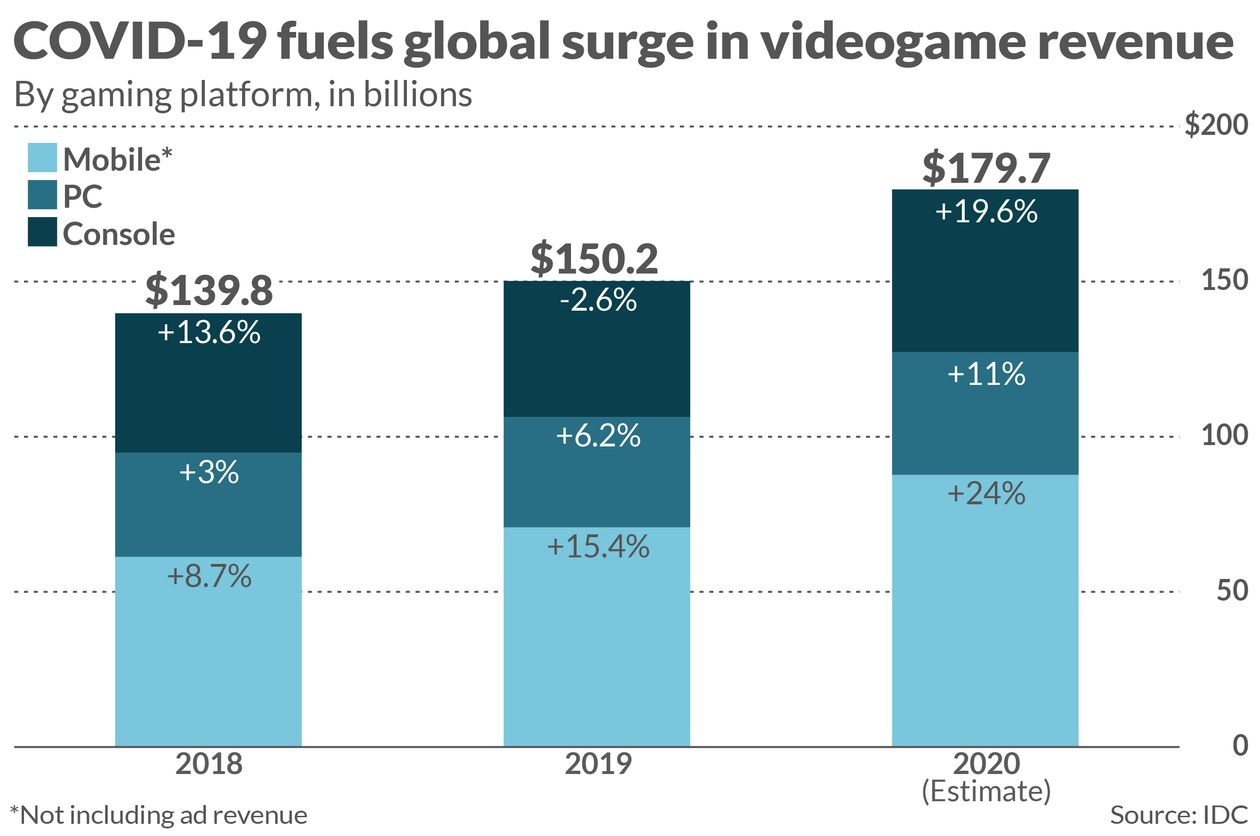
\includegraphics[width=0.5\textwidth]{images/videogamesMoney.jpeg}
    \caption{Ingressos dels videojocs. Font: \cite{VidogamesMoreMoney}}
    \label{fig:VideogamesRevenuesImage}
\end{figure}

\subsection{Termes i conceptes bàsics}
En aquest apartat s'explicaran termes i conceptes relacionats que apareixeran durant tot el transcurs del projecte i que poden donar lloc a la confusió o desconeixement del significat al lector.

\begin{itemize}
\item \textbf{Elo:} Es coneix com a Elo el sistema de puntuació creat pel físic estatunidenc d'origen hongarès Arpad Elo, que mesura els nivells d'habilitat relatius dels jugadors en els esports com els escacs o videojocs competitius com el League of Legends. \cite{wikipediaElo}

\item \textbf{Matchmaking:} S'anomena matchmaking a l'algorisme utilitzat en la majoria dels videojocs multijugador que tracta d'emparellar els jugadors o equips d'un nivell o habilitats similars per enfrontar-se entre ells, mitjançant l'anàlisi de les estadístiques d'aquests. \cite{matchmakingDef}.

\item \textbf{Videojoc competitiu:} S'entén com a videojoc competitiu un videojoc online, és a dir, que es juga a través d'Internet, on els jugadors competeixen entre ells, sigui en equip o individual, per ser uns millors que els altres. Un exemple d'aquests poden ser els escacs o els jocs de lluita, com el Street Fighters o Mortal Kombat.

\item \textbf{Habilitat del jugador:} Es coneix com a habilitat del jugador a la capacitat que té aquest per demostrar la seva destresa en un joc, és a dir, en altres paraules, com és d'hàbil jugant.
\end{itemize}

\newpage
\subsection{Identificació del problema}
Com s'ha vist anteriorment, els videojocs cada cop estan agafant més importància en la indústria: cada cop són més coneguts, es destinen més diners i en generen més. Per aquests motius, és molt important dissenyar-los bé i per fer-ho, s'han de tenir en compte molts aspectes, com per exemple la temàtica, els escenaris, els personatges, etc. Però també és molt important la jugabilitat, fer que sigui divertit i entretingut. A més, dintre dels jocs competitius, es necessita un bon sistema d'Elo i d'aparellament, per fer encara el videojoc més equilibrat i generar més rivalitat, tot i que també pot haver-hi interessos comercials.

Desenvolupar una bona fórmula de l'Elo equival, normalment, a representar el nivell d'habilitat del jugador i al seu progrés a l'hora de millorar. Per tant, s'ha d'estudiar rigorosament com fer-la i saber quines variables la modificaran (guanyar, perdre, morir més o menys, etc.).

També cal afegir que l'Elo pot ser molt diferent depenent de la situació en què es vulgui aplicar. Per exemple, si en un videojoc es fa un campionat setmanal, on es vol reduir el nombre de jugadors durant el transcurs d'aquest, es pot generar un algorisme que contempli un Elo molt variat entre els diferents participants al principi de la competició, però que sigui més similar cap al final. Per una altra banda, si es juga un campionat mensual on es vol que hi participin tots els jugadors i es desitja una classificació apropiada a l'Elo de cada un, es pot desenvolupar un algorisme que agrupi les partides mitjançant un Elo similar.

Com es pot observar, la fórmula de l'Elo pot ser molt variable i s'han de fer diverses proves per arribar a l'adequada. El problema és que no hi ha cap programa que permeti simular les diferents versions per saber quina és vàlida i quina no. El que s'ha de fer actualment és plantejar una simulació que s'adeqüi a l'algorisme i fer moltes partides per veure l'evolució. Això pot tenir conseqüències, i és que testejar i comparar els resultats de les diferents fórmules pot portar molt temps, el qual es podria invertir en altres aspectes del desenvolupament del videojoc. 

És per aquest motiu que és necessària una eina software per a les empreses desenvolupadores de jocs amb interès comercial, que els permeti simular partides amb l'algorisme d'Elo que se li introdueixi, sigui quin sigui, i permeti avaluar els resultats. D'aquesta manera, podran escollir quin s'adapta millor a la jugabilitat i progressió del joc.

\newpage
\subsection{Exemples de sistemes d'Elo en els videojocs}
L'Elo es pot calcular de diverses fórmules, des de la més simple que és la d'obtenir punts depenent de si es guanya o es perd, fins a la de contemplar el teu progrés en la partida, com per exemple si s'ha eliminat molts contrincants, si s'ha mort moltes vegades, etc. A continuació es mostraran alguns exemples de sistemes d'Elo utilitzars en videojocs molt coneguts:

\begin{itemize}
    \item \textbf{Escacs:} Els escacs consisteixen en partides d'u contra u on l'objectiu és eliminar el rei enemic. Aquest utilitza el mètode més senzill per calcular la puntuació d'Elo i és el següent: és mesura la probabilitat de guanyar al rival més la de fer taules (empatar). A partir d'aquí s'extreuen els punts d'Elo a guanyar o perdre depenent del resultat. La quantitat també depèn del rang on juguin la partida, com més rang tinguin, més punts guanyaran o perdran \cite{wikipediaElo}.
    \item \textbf{Rocket League:} El Rocket League és un videojoc de futbol, amb la diferència que en canvi de jugar amb persones, es juga amb cotxes. En aquest cas, l'Elo s'anomena MMR (MatchMaking Rank) i funciona similar al dels Escacs. Si es guanya al rival, s'obté MMR i si es perd, es resta. La quantitat pot variar depenent del rang en el qual es trobi el jugador i depenent del nivell de l'equip rival. En aquest cas, marcar gols, fer parades o assistències no contribueix a obtenir més Elo \cite{rocketElo}.
    \item \textbf{League of Legends:} El League of Legends o LOL és un joc per equips on l'objectiu és enderrocar una estructura anomenada Nexo que es troba en la base del rival. Aquest videojoc funciona per rangs i per pujar-ne d'un a un altre, has d'acumular una certa quantitat de LP (League Points). Aquests funcionen com els punts d'Elo explicats anteriorment: si el jugador guanya la partida, n'adquirirà més o menys depenent del nivell del rival. En canvi, si la perd, se li restaran. La diferència amb els videojocs anteriors és que un cop ha adquirit els LP suficients per pujar de rang, necessita jugar unes fases d'ascensió. Si les passa, pujarà de rang i tindrà els LP corresponents. En canvi, si les perd, els LP seran restablerts al del rang corresponent \cite{LolElo}.
    \item \textbf{Counter Strike: Global Offensive:} El Counter Strike: Global Offensive o CSGO és un videojoc per equips de diverses rondes on l'objectiu és eliminar a tot l'equip rival, o evitar que es planti la bomba o desactivar-la, o plantar-la i fer-la explotar, depenent del rol que tingui l'equip.  En aquest joc el sistema d'Elo funciona de manera diferent: cada ronda que es juga és com si fos una partida d'escacs. Els punts d'Elo es veuen repartits al final de cada una d'elles. La diferència està en el fet que aquest joc si contempla el nombre de morts que ha tingut un jugador, el número de baixes, si ha complert l'objectiu, etc. per repartir els punts d'Elo. També té molt en compte qui ha estat el MVP de la ronda, enduent-se una gran part dels punts \cite{csgoELO1} \cite{csgoELO2}. 
\end{itemize}

\newpage
\subsection{Motivació}
Els videojocs és un aspecte que m'ha apassionat tota la vida. Des de ben petit fins al dia d'avui que els porto jugant i gaudint. De fet, el quadrimestre passat vaig cursar l'assignatura de videojocs per tal de veure i entendre com funcionaven.

A l'hora d'escollir un tema per fer el TFG, vaig demanar ajuda a diversos professors que havia tingut durant la carrera per veure si em podien donar alguna idea. D'entre totes les propostes que havia rebut, les quals eren molt interessants, va haver-hi una que em va cridar molt l'atenció. Evidentment, aquesta és la del meu TFG i consisteix a fer un simulador d'Elo per estudiar aquest mateix i veure com evolucionava. Vaig escollir aquesta idea per dues raons: la primera és que era una temàtica sobre els videojocs, que com he mencionat anteriorment, m'agraden molt. La segona és que és un aspecte que mai m'havia plantejat com funcionava i que malauradament no s'havia estudiat en l'assignatura. Per tant, vaig escollir aquest TFG per augmentar el meu coneixement sobre els videojocs i com estan fets.


\newpage
\section{Competència en el mercat}
\subsection{Solucions existents}
El sistema d'Elo d'un videojoc és molt important, ja que ha de representar, normalment, el nivell d'habilitat del jugador i a més, aconseguir fer les partides entretingudes. Llavors, podem arribar a la conclusió de què ha d'estar ben fet perquè un joc triomfi. És per aquest motiu que he realitzat una recerca per Internet de programes que simulin i permetin configurar el sistema d'Elo d'un videojoc, però només he trobat repositoris de Github que ho simulen, donada una fórmula predeterminada, on a vegades es poden canviar algunes variables, o bé una pàgina web que fa el mateix. Els millors resultats obtinguts han estat els següents:

\begin{itemize}
    \item \textbf{Repositori de RemiFabre \cite{EloSystemRemi}:} En aquest repositori anomenat "Elo" \space es troba un programa fet en python que simula l'evolució de l'Elo en diversos jugadors amb puntuacions diferents. Aquest programa té dues modalitats, en la primera és que els jugadors només s'enfronten entre si una vegada rere l'altre, mentre que en la segona modalitat s'enfronten a jugadors creats només per aquella partida i amb un "winrate" \space fixat. L'algorisme de l'Elo està predeterminat i com a molt es pot canviar el valor de certes variables. Posteriorment, es mostra el resultat en una gràfica. 
    
    \item \textbf{Repositori de cardsorg \cite{EloSystemCardsorg}:} Aquest repositori de Github anomenat "Elo" \space inclou un software que simula l'enfrontament entre dos jugadors i diu el respectiu Elo de cadascú. Té tres funcionalitats diferents; la primera permet fer l'enfrontament entre dues persones amb l'Elo i el resultat que es vulguin assignar. També permet canviar el valor de la variable K, que és el màxim de punts que pot guanyar o perdre un jugador en una partida. La segona funcionalitat consisteix a mostrar la diferència entre els dos jugadors i la tercera fa el mateix, però també mostra la diferència estimada.
    
    \item \textbf{Repositori d'iain \cite{EloSystemiain}:} En aquest tercer repositori anomenat "Elo" \space es troba un altre programa que permet simular i modificar alguna variable del sistmea d'Elo. En aquest cas, es poden crear jugadors amb la puntuació desitjada i enfrontar-los entre si, decidint el resultat. També diu si són professionals o principiants depenent dels seus punts. Aquest software també permet diferents configuracions, com la modificació de la variable K, on es pot definir depenent del nombre de partides fetes. També permet modificar a partir de quina quantitat de punts es deixa de ser un principiant i amb quina puntuació comença un jugador.
    
    \item \textbf{Elo Calculator \cite{EloSystemOmnicalculator}:} Aquesta calculadora online de la pàgina web "Omnicalculator"\space permet calcular l'Elo d'un jugador després de fer diferents jocs i també modificar la variable K. Hi ha dos opcions a escollir: una única partida o múltiples d'elles. La calculadora deixa assignar els punts desitjats al jugador principal i a cada un dels seus rivals, permetent també escollir el resultat de cada enfrontament. Al final, mostra una taula amb quants punts s'han guanyat i perdut en cada joc i quina és la puntuació final.
\end{itemize}

\subsection{Justificació de la meva proposta}
Un cop vistes totes les solucions que hi ha actualment a Internet, podem concloure que totes elles tenen aspectes positius: permeten modificar la variable K,  mostren un gràfic de com va evolucionant l'Elo després de diverses partides,  permeten escollir el resultat de cada joc o ensenyen quants punts es guanyen o perden en cada un. Tot i això, totes elles estan lligades a la mateixa fórmula, i és aquesta la principal diferència amb el meu projecte.

La meva solució també permet modificar el valor de diverses variables, simular diverses partides i exportar els resultats per fer una gràfica, però el més important és que permetrà canviar l'algorisme per calcular l'Elo completament. Es podrà utilitzar l'algorisme que es desitgi, ja sigui el predeterminat o un creat per l'empresa o persona que dissenyi el videojoc, permetent així veure la comparativa entre les diferents fórmules i escollint la més adequada pel videojoc. A més, per tal de simular millors les partides, també permetrà canviar l'algorisme de com es juguen i també permetrà crear jugadors amb les característiques desitjades. Tot això fa el simulador més dinàmic i més adaptable, ajustant-se a la voluntat de l'empresa.

A continuació, per tal d'aclarir les diferències entre els diferents programes, en la taula \ref{tab:TaulaFuncionalitat} es pot observar una graella comparativa entre les diferents funcionalitats dels diversos programes trobats i el meu.

\begin{table}[H]
    \begin{center}
        \begin{tabular}{|l|c|c|c|c|c|}
            \hline
            \rowcolor[HTML]{9B9B9B} 
            {\color[HTML]{000000} \textbf{Funcionalitats}}                                  & {\color[HTML]{000000} \textbf{RemiFabre}}        & {\color[HTML]{000000} \textbf{cardsorg}}         & {\color[HTML]{000000} \textbf{iain}}             & {\color[HTML]{000000} \textbf{EloCalculator}}    & {\color[HTML]{000000} \textbf{El meu projecte}}  \\ \hline
            \begin{tabular}[c]{@{}l@{}}Fórmula d'ELO\\ determinada\end{tabular}             & {\color[HTML]{333333} \checkmark}                         & {\color[HTML]{333333} \checkmark}                         & {\color[HTML]{333333} \checkmark}                         & {\color[HTML]{333333} \checkmark}                         & {\color[HTML]{333333} \checkmark}                         \\ \hline
            \begin{tabular}[c]{@{}l@{}}Canviar variables\\ algorisme d'ELO\end{tabular}     & \cellcolor[HTML]{FFFFFF}{\color[HTML]{333333} \checkmark} & \cellcolor[HTML]{FFFFFF}{\color[HTML]{333333} \checkmark} & \cellcolor[HTML]{FFFFFF}{\color[HTML]{333333} \checkmark} & \cellcolor[HTML]{FFFFFF}{\color[HTML]{333333} \checkmark} & \cellcolor[HTML]{FFFFFF}{\color[HTML]{333333} \checkmark} \\ \hline
            \begin{tabular}[c]{@{}l@{}}Simulació amb gran\\ nombre de partides\end{tabular} & {\color[HTML]{333333} \checkmark}                         & {\color[HTML]{333333} X}                         & {\color[HTML]{333333} X}                         & {\color[HTML]{333333} X}                         & {\color[HTML]{333333} \checkmark}                         \\ \hline
            \begin{tabular}[c]{@{}l@{}}Personalitzar puntuació\\ de jugadors\end{tabular}   & {\color[HTML]{333333} X}                         & {\color[HTML]{333333} \checkmark}                         & {\color[HTML]{333333} \checkmark}                         & {\color[HTML]{333333} \checkmark}                         & {\color[HTML]{333333} X}                         \\ \hline
            \begin{tabular}[c]{@{}l@{}}Decidir resultat\\ d'un enfrontament\end{tabular}    & {\color[HTML]{333333} X}                         & {\color[HTML]{333333} \checkmark}                         & {\color[HTML]{333333} \checkmark}                         & {\color[HTML]{333333} \checkmark}                         & {\color[HTML]{333333} X}                         \\ \hline
            \begin{tabular}[c]{@{}l@{}}Mostrar resultat\\ en gràfiques\end{tabular}         & {\color[HTML]{333333} \checkmark}                         & {\color[HTML]{333333} X}                         & {\color[HTML]{333333} X}                         & {\color[HTML]{333333} X}                         & {\color[HTML]{333333} X}                         \\ \hline
            \begin{tabular}[c]{@{}l@{}}Personalitzar\\ algorisme d'ELO\end{tabular}         & {\color[HTML]{333333} X}                         & {\color[HTML]{333333} X}                         & {\color[HTML]{333333} X}                         & {\color[HTML]{333333} X}                         & {\color[HTML]{333333} \checkmark}                         \\ \hline
            \begin{tabular}[c]{@{}l@{}}Personalitzar\\ algorisme de partida\end{tabular}         & {\color[HTML]{333333} X}                         & {\color[HTML]{333333} X}                         & {\color[HTML]{333333} X}                         & {\color[HTML]{333333} X}                         & {\color[HTML]{333333} \checkmark}                         \\ \hline
            \begin{tabular}[c]{@{}l@{}}Personalitzar\\ creació de jugadors\end{tabular}         & {\color[HTML]{333333} X}                         & {\color[HTML]{333333} X}                         & {\color[HTML]{333333} X}                         & {\color[HTML]{333333} X}                         & {\color[HTML]{333333} \checkmark}                         \\ \hline
            \begin{tabular}[c]{@{}l@{}}Exportar dades\\ a Excel\end{tabular}                & {\color[HTML]{333333} X}                         & {\color[HTML]{333333} X}                         & {\color[HTML]{333333} X}                         & {\color[HTML]{333333} X}                         & {\color[HTML]{333333} \checkmark}                         \\ \hline
        \end{tabular}
        \caption{Taula comparativa de les diferents funcionalitats dels programes}
        \label{tab:TaulaFuncionalitat}
    \end{center}
\end{table}

\section{Abast}
En aquest apartat es comentaran els objectius que ha de tindre el projecte, igual que els requisits que ha de complir. També es contemplaran els obstacles i riscos que poden aparèixer durant tot el desenvolupament.

\subsection{Objectius}
L'objectiu principal d'aquest projecte és poder crear un programa software que permeti simular el càlcul de l'Elo en els videojocs i veure la seva evolució, per determinar si és un algorisme vàlid, per veure si l'Elo correspon al nivell del jugador i per veure si l'aparellament és el correcte. Però per aconseguir que el programa pugui complir amb aquestes funcionalitats, cal assolir un seguit de sub-objectius:
\begin{itemize}
    \item \textbf{Personalització de l'algorisme del sistema d'Elo:} El programa ha de permetre tant la modificació de variables com poder canviar la fórmula sencera, permetent així introduir qualsevol algorisme per veure el seu funcionament.
    
    \item \textbf{Simulació de partides:} El software ha de permetre simular partides per així poder aplicar la fórmula de l'Elo i poder comprovar que l'aparellament de jugadors és el correcte. S'ha de contemplar que poden haver-hi variables que poden afectar al resultat de la partida, per exemple un jugador pot tenir un arma millor que l'altre, una armadura més resistent, un millor cotxe, etc. També ha de tenir en compte la diferència d'habilitat entre els contrincants, el resultat esperat vs. el real i la quantitat de punts d'Elo guanyats o perduts per cada partida. 
    
    \item \textbf{Comparar resultats entre diferents variables i algorismes:} Per poder determinar si la fórmula de l'Elo és la correcta, cal poder comparar els resultats entre els diferents algorismes. És per aquest motiu que es guardaran les dades i es permetrà exportar-les a l'Excel, per poder analitzar-les i comparar-les.
\end{itemize}

A la figura \ref{fig:EsquemaObjectius} es pot observar un esquema dels diversos objectius i subojectius del programa.

\begin{figure}[H]
    \centering
    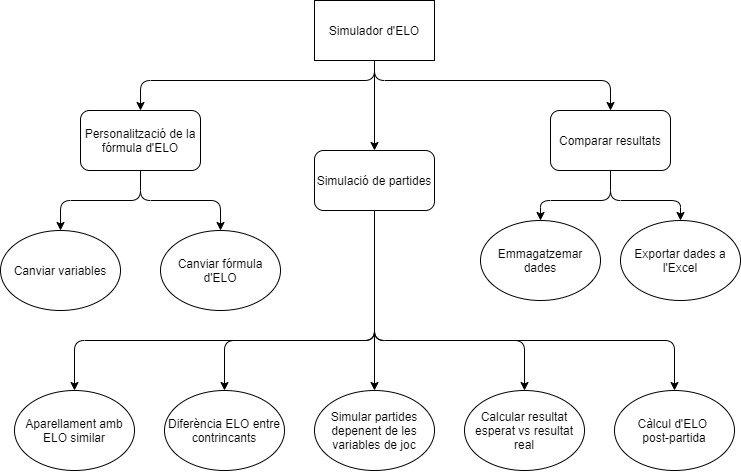
\includegraphics[width=0.9\textwidth]{images/FuncionsEsquema.jpg}
    \caption{Esquema dels objectius i subobjectius del sistema. Font: Elaboració pròpia}
    \label{fig:EsquemaObjectius}
\end{figure}

\subsection{Obstacles i riscos}
Durant tot el transcurs del projecte poden aparèixer diversos obstacles i riscos que poden alentir el desenvolupament del projecte. Per aquest motiu, cal identificar-los i saber-ne d'ells.

\begin{itemize}
    \item \textbf{Data d'entrega fixa:} El TFG té una data límit fixada i, per tant, que s'ha de complir. Però els possibles problemes que ens podem trobar durant el desenvolupament del projecte poden generar endarreriments i, per tant, empitjorar la qualitat del programa o eliminar alguna funció no essencial per falta de temps.
    \item \textbf{Desconeixement en simulació:} Un aspecte fonamental del programa és la simulació de partides. Però a causa del meu desconeixement en l'àmbit de la simulació dins la informàtica, és probable que es generin endarreriments i possibles errors a l'hora de programar.
    \item \textbf{Desconeixement en les tecnologies emprades:} A causa del meu desconeixement sobre el llenguatge Lua o sobre el poc ús fet de QT, és probable que s'alenteixi el desenvolupament del projecte, ja que hauré d'aprendre a utilitzar-los correctament.
    \item \textbf{Bugs i errors:} Durant tot el transcurs de programar i testejar el programa, poden aparèixer diferents errors i bugs que em poden fer perdre molt temps, i per tant, endarrerir el desenvolupament.
\end{itemize}


\newpage
\section{\textit{Stakeholders}}
Els \textit{Stakeholders} són una part fonamental pel desenvolupament del projecte, ja que són totes aquelles persones o organitzacions afectades pel producte a crear i que tenen interès en aquest, ja sigui de forma directa o indirecta. A continuació es llistaran les parts interessades del software a desenvolupar.

\begin{itemize}
    \item \textbf{Empreses de videojocs:} Les empreses desenvolupadores de videojocs es veuran principalment afectades pel projecte. Si el sistema d'Elo aplicat al producte és bo, hi ha més possibilitats de que el joc triomfi. Per tant, quan més èxit tingui el joc, més conegut serà, més jugadors captarà i més beneficis obtindrà l'empresa.
    
    \item \textbf{Jugadors:} Els jugadors de videojocs són les principals parts interessades i són les més importants. Aquests es veuran implicats de forma indirecte, ja que són els que jugaran i seran puntuats pel sistema d'Elo resultant. També són qui han de trobar el joc entretingut i divertit, ja que seran els encarregats de fer que aquest tingui èxit. 
    
    \item \textbf{Desenvolupadors de videojocs:} Els desenvolupadors de videojocs són qui utilitzaran el software de forma directe. Seran els encarregats d'estudiar i plantejar les diferents fórmules del sistema d'Elo i simular-les en l'eina a desenvolupar, per així decidir quina d'elles s'adapta més al videojoc i farà que hi hagi una millor experiència.
    
    \item \textbf{Propietari del TFG:} Jo mateix soc un dels principals \textit{steakeholders} del projecte, ja que seré l'únic desenvolupador. El meu objectiu serà fer-lo de la millor forma possible i eficient, testejar-lo i documentar tot el procés.
    
\end{itemize}

\newpage
\section{Requisits del sistema}
Per tal d'assolir el bon funcionament del sistema i complir tots els objectius mencionats prèviament, aquest projecte ha d'assolir un seguit de requisits funcionals i no funcionals que es mostraran a continuació.

\subsection{Requisits funcionals}
El simulador que es desenvolupa en aquest treball disposa d'un seguit de requisits funcionals que permeten a l'usuari fer-ne ús del sistema. Seguidament, s'enumeraran cada un d'ells:

\begin{itemize}
    \item \textbf{Entrada de fitxers Lua:} El programa ha de permetre poder carregar un fitxer de script en Lua que contingui diverses característiques i funcions per poder personalitzar la simulació, com l'algorisme del sistema d'Elo o les característiques dels jugadors.
    
    \item \textbf{Configuració de la fórmula del sistema d'Elo:} El sistema ha de poder entendre i executar perfectament la fórmula d'Elo que hagi introduït l'usuari mitjançant el script de Lua. 
    
    \item \textbf{Configuració de la fórmula per jugar la partida:} El sistema ha de poder llegir i executar la fórmula de joc de les partides per tindre en compte totes les propietats que vol l'usuari.
    
    \item \textbf{Creació dels jugadors per fer les simulacions:} El sistema ha de crear el nombre de jugadors necessaris per poder executar la simulació. Cada un d'ells ha de tenir les característiques introduïdes per l'usuari.
    
    \item \textbf{Configuració de les característiques dels jugador:} L'usuari ha de ser capaç de modificar les característiques o propietats que han de tenir els jugadors mitjançant el fitxer Lua.
    
    \item \textbf{Creació d'equips:} El sistema ha de permetre crear equips tenint en compte les dades introduïdes per l'usuari respecte la diferència d'Elo entre jugadors i el nombre de membres d'un equip. Tot equip tindrà una diferència màxima inferior o igual a l'especificada i tindrà un nombre de components idèntics a l'indicat.
    
    \item \textbf{Creació de les partides:} El sistema ha de permetre crear partides tenint en compte la diferència màxima d'Elo que pot haver-hi entre els dos equips. Aquesta dada haurà estat introduïda per l'usuari prèviament.
    
    \begin{comment}
    \item \textbf{Matchmaking:} L'eina a desenvolupar ha de ser capaç d'aparellar els diversos jugadors segons la diferència d'Elo demanada, per poder simular posteriorment les partides.
    \end{comment}
    
    \item \textbf{Simulació d'una partida:} El sistema ha de simular una partida entre els equips i determinar un resultat. Per fer-ho, tindrà en compte el sistema implementat per l'usuari en el fitxer Lua.
    
    \item \textbf{Càlcul de l'Elo:} El software ha de permetre poder executar l'algorisme de l'Elo i modificar la puntuació de cada un dels jugadors de la forma adequada.
    
    \item \textbf{Configuració de la simulació:} El sistema ha de permetre la configuració d'una sèrie de variables per fer la simulació, concretament: el nombre de jugadors, el nombre de components d'un equip, el nombre de partides a simular,  la diferència de puntuació entre els jugadors d'un equip i un enfrontament i la destinació de les estadístiques.
    
    \item \textbf{Emmagatzematge de dades:} El software ha de poder emmagatzemar les dades extretes de les simulacions per poder-les utilitzar i actualitzar més tard.
    
     \item \textbf{Sortida de fitxers Excel:} L'eina a desenvolupar ha de poder permetre exportar les dades obtingudes a un fitxer Excel per així poder-les analitzar i comparar.
\end{itemize}

\subsection{Requisits no funcionals}
Pel que fa als requisits no funcionals, ens centrarem en el rendiment de l'aplicació i la usabilitat per l'usuari.

\begin{itemize}
    \item \textbf{Facilitat d'ús:} El programa ha de ser intuïtiu i simple per a que qualsevol persona el pugui utilitzar.
    
    \item \textbf{Aprenentatge:} El software ha de ser fàcil d'aprendre per a qualsevol usuari.
    
    \item \textbf{Eficiència:} El programa ha de ser eficient degut a la gran quantitat de simulacions que ha de fer, per tant, ha d'anar el més ràpid possible.
    
    \item \textbf{Aparença:} L'eina ha de ser atractiva visualment pels usuaris que l'utilitzin. 
\end{itemize}

\newpage
\section{Metodologia i rigor}
La metodologia que es durà a terme per desenvolupar el projecte és un aspecte molt important a tenir en compte, ja que pot canvia per complet com evolucionarà. Hi han dues grans metodologies: la cascada o \textit{waterfall} i l'\textit{agile}.

La primera, l'anomenada \textit{waterfall} és la més tradicional. Aquesta té en compte els \textit{stakeholders} i clients al principi del projecte, i després es desenvolupa un pla seqüencial per satisfer els seus requisits. S'anomena d'aquesta manera perquè cada fase del pla proposat passa a la següent un cop s'ha acabat l'anterior \cite{waterfallModel}.

La metodologia cascada és utilitzada quan els requeriments estan molt clars i fixes, quan la definició del producte és estable, quan la tecnologia no evoluciona constantment i quan el projecte és curt \cite{waterfallTutorialsPoint}.

Per una altra part, la metodologia \textit{agile} consisteix en una contínua iteració de desenvolupament i testeig del software on s'interacciona de forma contínua amb els clients i \textit{stakeholders} per saber el seu \textit{feedback} \cite{agileVsWaterfall}.

Aquesta és utilitzada per projectes llargs on es vol el \textit{feedback} del client constantment, quan es vol treballar amb tecnologies en evolució continua, també quan els requeriments no estan clars i poden canviar freqüentment, igual que la definició del producte. Com es pot observar, és la contrapart de la metodologia \textit{waterfall}. 

Per tant, un cop explicades les dues metodologies, es pot observar que el meu projecte s'assimila a les condicions de la primera metodologia. El període de temps és curt, ja que el TFG dura entre tres i quatre mesos, i els requeriments ja estan definits, igual que el producte.

Llavors, un cop decidida la metodologia, s'ha d'explicar com funciona. Com bé es pot observar en la figura \ref{fig:WaterfallImage}, aquesta metodologia consta de sis fases. La primera d'elles s'anomena "Requeriments", i és on s'especifiquen i redacten tots els requeriments. La segona s'anomena "Disseny", i és on s'especifica el disseny del sistema i la seva arquitectura. La següent és la fase de "Desenvolupament", on el programa és dividit en petites unitats on cada una farà una funcionalitat i la testejarà. Posteriorment ve la fase de "Testeig", on s'ajunta tot el codi fet per cada una de les unitats anteriors i es testeja el resultat. Seguidament es troben els errors i es solucionen. La següent fase és la de "Desplegament", on el producte es llença al mercat o és entregat al client. Finalment hi ha la fase de "Manteniment", on es manté i millora el programa \cite{waterfallImage}. 

\begin{figure}[H]
    \centering
    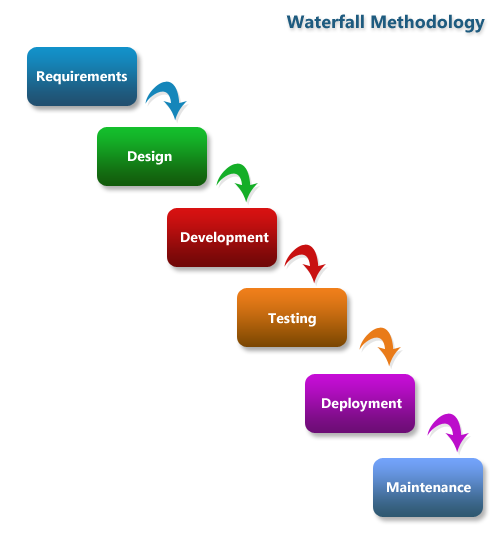
\includegraphics[width=0.5\textwidth]{images/Waterfall-Metodology.png}
    \caption{Fases de la metodologia \textit{Waterfall}. Font: \cite{waterfallImage}}
    \label{fig:WaterfallImage}
\end{figure}

\subsection{Control de versions}

Durant el desenvolupament del projecte s'utilitzarà Git\cite{git} per poder realitzar diferents versions d'aquest. També s'utilitzarà Github\cite{Github} per pujar tot el codi del projecte i tota la documentació necessària. D'aquesta manera, el director podrà veure el progrés i podrà analitzar com s'està implementant la solució. Addicionalment, és podrà consultar i accedir a qualsevol versió anterior.

\subsection{Control de seguiment}
    
Durant el transcurs de tot el TFG, Google Meet \cite{GoogleMeet} serà utilitzat per mantenir al director informat i poder-li comentar qualsevol dubte o error. S'ha acordat fer, sempre que sigui possible i necessari, una reunió per setmana. D'aquesta manera es podrà discutir el progrés del projecte i observar si es va pel bon camí.

\subsection{Control de tasques}

El Trello\cite{Trello} s'utilitzarà tenir estructurades les diverses tasques a realitzar durant el projecte. Cada gran funcionalitat estarà descomposta per petites tasques per tal de facilitar la implementació. A més, es faran quatre columnes per organitzar bé l'estat del projecte: TO DO, DOING, READY, DONE.

\newpage
\section{Implementació}
\subsection{Tecnologies utilitzades}
Per dur a terme aquest projecte s'han escollit un seguit d'eines i tecnologies que facilitaran el seu desenvolupament. A continuació s'explicaran cada una d'elles i el motiu de la seva elecció.

\subsubsection{Llenguatges de programació}
\begin{itemize}
    \item \textbf{C++:} El projecte s'ha desenvolupat en C++ per dos motius. El primer de tots és que és el llenguatge que he utilitzat més freqüentment i per tant, el que tinc més fresc, ja que és el que vaig utilitzar per a l'assignatura de Videojocs el quadrimestre anterior. El segon motiu és la gran facilitat que hi ha a Internet per trobar informació sobre com funcionen certs aspectes o mètodes del llenguatge, o per consultar dubtes o erros que puguin sorgir durant el desenvolupament. 
    \item \textbf{Lua:} Lua és un llenguatge de programació de scrip potent, eficient i lleuger que pot ser integrat dins d'altres softwares o pot ser compilat en qualsevol d'ells sempre que estigui basat en aquest llenguatge C, ja que és com està fet l'intèrpret \cite{luaAbout}. S'ha escollit aquest llenguatge perquè és fàcil d'aprendre i d'utilitzar i perquè també hi ha la suficient documentació i resolució de problemes a Internet.
    \item \textbf{\LaTeX:} \LaTeX és un software lliure i és un sistema de composició de textos, normalment utilitzat per escriure documents i articles científics \cite{wikipediaLatex}. S'ha escollit \LaTeX per fer la memòria perquè és un llenguatge còmode per escriure una documentació llarga i clara, ja que ajuda a estructurar el format de forma més senzilla.
\end{itemize}

\subsubsection{Eines}
\begin{itemize}
    \item \textbf{QT:} QT és una eina que utilitzarem per desenvolupar la interfície gràfica del programa. Ha estat una eina utilitzada durant alguna assignatura de la carrera, per tant, ja es té cert coneixement sobre ella i és per això que s'ha escollit. 
    \item \textbf{Visual Studio 2019:} Visual Studio és una IDE compatible amb diversos llenguatges de programació com C++ o C\#. S'ha escollit aquesta eina per desenvolupar el programa perquè ja l'havia utilitzat anteriorment, i per tant, ja sé com funciona.  
    \item \textbf{Overleaf:} Overleaf és l'editor de text que s'utilitzarà per escriure en \LaTeX.
    \item \textbf{Git:} Git és un software de control de versions per manejar des de petits fins a grans projectes \cite{git}. Aquesta eina ens serà útil per emmagatzemar tot el codi del nostre programa i poder anar fent versions del propi.
    \item \textbf{Github \cite{Github}:} Github és un servei de repositoris que utilitza les versions Git. Serà emprat per guardar i compartir el codi i la documentació feta durant tot el projecte. Té l'avantatge de què es poden accedir a versions anteriors del codi i també gestionar els errors i bugs trobats. 
    \item \textbf{Google Meet \cite{GoogleMeet}:} Google Meet és un servei de Google que serveix per fer videotrucades. Aquesta eina serà utilitzada per mantenir al director informat i poder-li comentar qualsevol dubte o error. S'ha acordat fer, sempre que sigui possible i necessari, una reunió per setmana. D'aquesta manera es podrà discutir el progrés del projecte i observar si es va pel bon camí.
    \item \textbf{Trello \cite{Trello}:} Trello és una eina per gestionar els projectes i les seves tasques. Serà utilitzada per apuntar les diverses funcions que s'han de realitzar i així saber quines s'estan fent, quines s'han de fer i quines s'han realitzat del tot. D'entre totes les eines que hi ha per fer un control de tasques, s'ha escollit aquesta perquè ja s'ha utilitzat prèviament en la carrera i és senzilla d'utilitzar.
\end{itemize}

\newpage
\section{Planificació temporal}
Planificar bé un projecte és molt important, ja que et permet gestionar el temps per desenvolupar tot el producte i preveure tots els errors que puguin sorgir. Concretament, aquest TFG té una duració aproximada de quatre mesos i mig, començant a mitjans de febrer, per ser exactes el dia 15, i finalitzant l'última setmana de juny. S'estima que la duració del treball sigui de 450 hores, que es distribuiran entre les 18 setmanes lectives (excloent Setmana Santa). Això equival a 25 hores per setmana, que fa una mitjana de 5 hores per cada dia lectiu. 

Durant el curset de GEP, es fa una planificació completa del TFG per tal d'assolir tots els objectius. En el meu cas, aquesta va ser molt completa, però no perfecte. La gran majoria de tasques s'han seguit tal com estaven organitzades, però hi ha hagut uns petits canvis. Bàsicament, s'ha afegit una tasca que consisteix a implementar totes les funcionalitats del sistema, però de forma molt bàsica, és a dir, sense llegir fitxers d'entrada ni aplicar cap algorisme, sinó fent-ho tot aleatori. En altres paraules, consisteix a fer tota l'estructura del programa. Aquesta decisió s'ha pres perquè d'aquesta manera, si hi ha algun inconvenient durant el desenvolupament, es tingui un producte funcional el dia de l'entrega. Igualment, aquesta tasca no ha afectat de forma negativa a les altres, ja que el temps que s'ha trigat a desenvolupar-la és temps estalviat en les futures tasques, simplement perquè l'estructura ja està feta.

Llavors, un cop comentat el canvi, ja es pot procedir en veure tota la planificació feta per aquest treball.

\subsection{Descripció de tasques}
Aquest projecte es pot dividir en tres grans parts, on cada una d'elles constarà de diverses tasques: gestió del projecte, desenvolupament i documentació i seguiment.
\subsubsection{Gestió del projecte}
\begin{itemize}
    \item \textbf{GdP1 - Contextualització i abast:} Es farà un document on es definirà la idea del treball, on s'identificaran els \textit{stakeholders}, s'analitzaran els programes similars, s'estudiaran els requisits i inconvenients que poden haver-hi i es descriurà la metodologia utilitzada. Tindrà una duració de 25 hores i serà necessari un ordinador amb Internet i l'Overleaf.
    \item \textbf{GdP2 - Planificació temporal:} S'escriurà un document on s'identificaran, es descriuran i s'organitzaran les diferents tasques que componen el projecte. També inclourà un diagrama de Gantt i la gestió dels diferents riscos que poden sorgir. Tindrà una duració de 10 hores i es necessitarà un ordinador amb connexió a Internet, l'Overleaf i el GanttProject. La tasca dependrà de GdP1.
    \item \textbf{GdP3 - Pressupost i sostenibilitat:} Es redactarà un document on es farà un pla econòmic del projecte i es farà un informe de sostenibilitat. Tindrà una durada de 15 hores i serà necessari un ordinador amb Internet, l'Overleaf i l'Excel. La tasca dependrà de GdP2.
    \item \textbf{GdP4 - Integració del document final:} Document on s'unificaran les tres tasques anteriorment explicades amb les correccions necessàries en cada una d'elles. S'estima una duració de 20h i serà necessari un ordinador amb connexió a Internet i l'Overleaf. La tasca dependrà de GdP3.
\end{itemize}

\subsubsection{Desenvolupament}
Dins del desenvolupament, podem dividir les tasques en uns altres tres grans grups, depenent de quin objectiu principal formen part: personalització de l’algorisme del sistema d’Elo, simulació de partides o comparar resultats entre diferents variables i algorismes.

\subsubsubsection{Personalització de l’algorisme del sistema d’Elo}
\begin{itemize}
    \item \textbf{PA1 - Preparació pel desenvolupament:} S'instal·laran tots els programes i IDEs necessaris per a poder desenvolupar el projecte. També es crearà el repositori de Github i es dissenyarà l'estructura del programa. Es necessitarà un ordinador amb connexió a Internet, l'IDE anomenat Visual Studio (VS), Github i el Visual Paradigm. Durarà 10 hores.
    \item \textbf{PA2 - Creació de l'estructura del programa:} Es crearà tota l'estructura del programa de la forma més senzilla, és a dir aplicant números aleatoris on sigui necessari i sense cap algorisme. També s'exportaran les dades de la forma més senzilla possible. Tindrà una durada 50 hores i serà necessari un ordinador amb connexió a Internet, Github i el Visual Studio. La tasca dependrà de PA3.
    \item \textbf{PA3 - Disseny d'algorisme d'Elo clàssic:} Es dissenyarà un algorisme d'Elo clàssic en un script de Lua per poder realitzar posteriorment l'execució del programa. Tindrà una durada 5 hores i serà necessari un ordinador amb Internet, Github, el Visual Studio i Lua. La tasca dependrà de PA2.
    \item \textbf{PA4 - Introducció i lectura de Fitxers Lua:} Es permetrà carregar un fitxer de script en Lua que contingui l'algorisme de l'Elo i s'haurà de poder executar. Tindrà una durada 15 hores i es necessitarà un ordinador amb Internet, el Github, el Visual Studio i Lua. La tasca dependrà de PA3.
    \item \textbf{PA5 - Interpretació de l'algorisme d'Elo:} S'haurà d'interpretar l'algorisme d'Elo introduït mitjançant el script en Lua per així saber quines variables s'utilitzen i quines s'han de tenir en compte. Tindrà una durada 35 hores i serà necessari un ordinador amb connexió a Internet, Github i el Visual Studio. La tasca dependrà de PA4.
\end{itemize}
\subsubsubsection{Simulació de partides}
\begin{itemize}
    \item \textbf{SP1 - Creació de jugadors:} S'hauran de crear els diversos jugadors que participaran en la simulació. Per cada un s'hauran d'afegir les diverses habilitats que poden afectar al resultat de la partida i al càlcul de l'Elo. Tindrà una durada de 30 hores i requerirà un ordinador amb Internet, Github i el Visual Studio. La tasca dependrà de PA5.
    \item \textbf{SP2 - Simulació de partida:} Es simularà una partida entre dos equips. Es tindran en compte tant l'Elo com les habilitats de cada un per decidir el resultat. Tindrà una durada 25 hores i serà necessari un ordinador amb Internet, Github i el Visual Studio. La tasca dependrà de SP1.
    \item \textbf{SP3 - Càlcul de l'Elo resultant:} Es calcularà i modificarà l'Elo de cada un dels jugadors depenent del resultat de la partida i de les estadístiques de cada un d'ells. Per fer-ho, s'utilitzarà l'algorisme introduït en el script de Lua. Tindrà una durada de 15 hores i es necessitarà un ordinador amb Internet, Github i el Visual Studio . La tasca dependrà de SP2.
    \item \textbf{SP4 - Disseny de l'algorisme de creació d'equips:} Es dissenyarà l'algorisme per aparellar els diferents jugadors en equips d'un Elo similar. Tindrà una durada de 15 hores i serà necessari un ordinador amb Internet, Github i el Visual Studio. La tasca dependrà de SP1.
    \item \textbf{SP5 - Disseny de l'algorisme de preparació de partides:} Es dissenyarà un algorisme que seleccionarà dos equips amb un nivell d'Elo similar per a que simulin una partida. S'empraran 5 hores per fer la tasca i requerirà un ordinador amb Internet, Github i el Visual Studio. Dependrà de SP4.
    \item \textbf{SP6 - Creació d'una simulació:} S'haurà de crear una simulació que permeti simular les diverses partides a realitzar. Es podran modificar elements com el número de jugadors, el número de partides que s'han de fer o la diferència màxima d'Elo entre un equip i un altre. Tindrà una durada de 10 hores i es requerirà d'un ordinador amb connexió a Internet, de Github i del Visual Studio. La tasca dependrà de SP5. 
\end{itemize}
\subsubsubsection{Comparar resultats entre diferents variables i algorismes}
\begin{itemize}
    \item \textbf{CR1 - Creació d'estructura de dades:} S'haurà de crear l'estructura per emmagatzemar les diferents dades de les partides i dels jugadors, per poder-les analitzar i utilitzar després. Tindrà una durada de 10 hores i serà necessari un ordinador amb connexió a Internet, Github i el Visual Studio. La tasca dependrà de SP6.
    \item \textbf{CR2 - Disseny de la interfície gràfica:} S'haurà de dissenyar una interfície gràfica simple i senzilla per facilitar a l'usuari l'ús del programa. Tindrà una durada de 40 hores i requerirà d'un ordinador amb connexió a Internet, de Github i del Visual Studio. La tasca dependrà de CR1. 
    \item \textbf{CR3 - Exportació de dades a l'Excel:} S'exportaran les dades emmagatzemades en l'estructura de dades en un fitxer amb format Excel, per així poder-les analitzar amb millor precisió. Les dades s'hauran de mostrar d'una forma entenedora i còmode per l'usuari. Tindrà una durada de 5 hores i es requerirà d'un ordinador amb Internet, de Github i del Visual Studio. La tasca dependrà de CR2.
\end{itemize}

\subsubsection{Documentació i seguiment}
\begin{itemize}
    \item \textbf{DS1 - Documentar la memòria:} Es redactarà la memòria de tot el desenvolupament del projecte. La tasca durarà 75 hores i serà necessari un ordinador amb Internet i l'Overleaf.
    \item \textbf{DS2 - Reunió setmanal:} Es realitzarà una reunió setmanal amb el director del projecte, Manel Rello, per parlar de l'evolució d'aquest i dels problemes o dubtes que puguin sorgir. Posteriorment s'afegirà a la memòria els detalls de cada reunió. En total, s'estima una durada de 25 hores i es requerirà un ordinador amb Internet, l'Overleaf i el Google Meet.
    \item \textbf{DS3 - Preparació de la presentació final:} Es prepararà l'exposició per a la presentació final del projecte que es farà davant un tribunal. Tindrà una durada de 10 hores i requerirà d'un ordinador amb connexió a Internet i d'un programa per fer diapositives. La tasca dependrà de DS1. 
\end{itemize}

\newpage
\subsection{Recursos humans}
S'entén com a recursos humans a totes aquelles persones que han d'ocupar un càrrec en el projecte per poder-lo dur a terme. Per fer-ho, cada una tindrà un rol i treballarà més o menys depenent de les tasques descrites prèviament en el diagrama de Gantt. A continuació es nomenaran cada un d'ells i s'explicarà la seva funció:
\begin{itemize}
    \item \textbf{Cap de projecte (CP):} El cap de projecte s'encarrega de gestionar el projecte. Gestiona els equips, planifica les tasques, calcula els pressupostos i els recursos necessaris i gestiona els riscos. També s'encarrega d'escriure la documentació.
    
    \item \textbf{Analista programador (AP):} L'analista programador té la funció d'identificar els requisits del sistema, de garantir la qualitat del programa i de dissenyar l'estructura del programa.
    
    \item \textbf{Arquitecte del Software (AS):} L'arquitecte del Software és la persona que escull quina tecnologia s'utilitzarà i realitza processos d'avaluació contínuament per veure que es compleixen els requisits.
    
    \item \textbf{Dissenyador d'UI (DUI):} El dissenyador d'interfícies gràfiques és qui s'encarrega de dissenyar l'apartat visual del programa per a que sigui simple d'utilitzar i clar. 
    
    \item \textbf{Programador (P):} El programador s'encarrega de programar el programa per a que funcioni.
    
    \item \textbf{Tester (T):} El tester té el paper de dissenyar diferents jocs de prova per comprovar el funcionament correcte del programa i detectar els errors.
\end{itemize}

\newpage
\section{Estimacions i Gantt}
\subsection{Estimacions}
\begin{table}[H]
    \small
    \begin{center}
        \begin{tabular}{|c|c|c|c|c|c|}
            \hline
            \rowcolor[HTML]{C0C0C0} 
            {\color[HTML]{000000} \textbf{ID}}                                                  & {\color[HTML]{000000} \textbf{Tasca}}                                                                             & {\color[HTML]{000000} \textbf{\begin{tabular}[c]{@{}c@{}}Durada \\ (hores)\end{tabular}}} & {\color[HTML]{000000} \textbf{Dependències}} & {\color[HTML]{000000} \textbf{\begin{tabular}[c]{@{}c@{}}RR \\ Materials\end{tabular}}}           & {\color[HTML]{000000} \textbf{\begin{tabular}[c]{@{}c@{}}RR\\ Humans\end{tabular}}} \\ \hline
            \rowcolor[HTML]{C0C0C0} 
            {\color[HTML]{000000} \textbf{GdP}}                                                 & {\color[HTML]{000000} \textbf{Gestió de projecte}}                                                                & {\color[HTML]{000000} \textbf{70}}                                                        & {\color[HTML]{000000} \textbf{}}             & \multicolumn{1}{l|}{\cellcolor[HTML]{C0C0C0}{\color[HTML]{000000} \textbf{}}}                     & \multicolumn{1}{l|}{\cellcolor[HTML]{C0C0C0}{\color[HTML]{000000} \textbf{}}}       \\ \hline
            {\color[HTML]{000000} GdP1}                                                         & {\color[HTML]{000000} Contextualització i abast}                                                                  & {\color[HTML]{000000} 25}                                                                 & {\color[HTML]{000000} }                      & {\color[HTML]{000000} PC, Overleaf}                                                               & {\color[HTML]{000000} CP}                                                           \\ \hline
            {\color[HTML]{000000} GdP2}                                                         & {\color[HTML]{000000} Planificació temporal}                                                                      & {\color[HTML]{000000} 10}                                                                 & {\color[HTML]{000000} GdP1}                  & {\color[HTML]{000000} \begin{tabular}[c]{@{}c@{}}PC, Overleaf, Gantt-\\ Project\end{tabular}}     & {\color[HTML]{000000} CP}                                                           \\ \hline
            {\color[HTML]{000000} GdP3}                                                         & {\color[HTML]{000000} Pressupost i sostenibilitat}                                                                & {\color[HTML]{000000} 15}                                                                 & {\color[HTML]{000000} GdP2}                  & {\color[HTML]{000000} PC, Overleaf, Excel}                                                        & {\color[HTML]{000000} CP}                                                           \\ \hline
            {\color[HTML]{000000} GdP4}                                                         & {\color[HTML]{000000} \begin{tabular}[c]{@{}c@{}}Integració del document\\ final\end{tabular}}                    & {\color[HTML]{000000} 20}                                                                 & {\color[HTML]{000000} GdP3}                  & {\color[HTML]{000000} PC, Overleaf}                                                               & {\color[HTML]{000000} CP}                                                           \\ \hline
            \rowcolor[HTML]{C0C0C0} 
            {\color[HTML]{000000} \textbf{D}}                                                   & {\color[HTML]{000000} \textbf{Desenvolupament}}                                                                   & {\color[HTML]{000000} \textbf{270}}                                                       & {\color[HTML]{000000} \textbf{}}             & {\color[HTML]{000000} \textbf{}}                                                                  & {\color[HTML]{000000} \textbf{}}                                                    \\ \hline
            {\color[HTML]{000000} PA1}                                                          & {\color[HTML]{000000} \begin{tabular}[c]{@{}c@{}}Preparació pel desenvolu-\\ pament\end{tabular}}                 & {\color[HTML]{000000} 10}                                                                 & {\color[HTML]{000000} }                      & {\color[HTML]{000000} \begin{tabular}[c]{@{}c@{}}PC, Github, VS, Visual \\ Paradigm\end{tabular}} & {\color[HTML]{000000} AP, AS, P, T}                                                 \\ \hline
            {\color[HTML]{000000} PA2}                                                          & {\color[HTML]{000000} \begin{tabular}[c]{@{}c@{}}Creació de l'estructura\\ del programa\end{tabular}}                & {\color[HTML]{000000} 50}                                                                 & {\color[HTML]{000000} PA1}                   & {\color[HTML]{000000} PC, Github, VS}                                                        & {\color[HTML]{000000} AP, AS, P, T}                                                 \\ \hline
            {\color[HTML]{000000} PA3}                                                          & {\color[HTML]{000000} \begin{tabular}[c]{@{}c@{}}Disseny d'algorisme d'Elo\\ clàssic\end{tabular}}                & {\color[HTML]{000000} 5}                                                                 & {\color[HTML]{000000} PA2}                   & {\color[HTML]{000000} PC, Github, VS, Lua}                                                        & {\color[HTML]{000000} AP, AS, P, T}                                                 \\ \hline
            {\color[HTML]{000000} PA4}                                                          & {\color[HTML]{000000} \begin{tabular}[c]{@{}c@{}}Introducció i lectura de \\ Fitxers Lua\end{tabular}}            & {\color[HTML]{000000} 15}                                                                 & {\color[HTML]{000000} PA3}                   & {\color[HTML]{000000} PC, Github, VS, Lua}                                                        & {\color[HTML]{000000} AP, AS, P, T}                                                 \\ \hline
            {\color[HTML]{000000} PA5}                                                          & {\color[HTML]{000000} \begin{tabular}[c]{@{}c@{}}Interpretació de l'algorisme\\ d'Elo\end{tabular}}               & {\color[HTML]{000000} 35}                                                                 & {\color[HTML]{000000} PA4}                   & {\color[HTML]{000000} PC, Github, VS}                                                             & {\color[HTML]{000000} AP, AS, P, T}                                                 \\ \hline
            {\color[HTML]{000000} SP1}                                                          & {\color[HTML]{000000} Creació de jugadors}                                                                        & {\color[HTML]{000000} 30}                                                                 & {\color[HTML]{000000} PA5}                   & {\color[HTML]{000000} PC, Github, VS}                                                             & {\color[HTML]{000000} AP, AS, P, T}                                                 \\ \hline
            {\color[HTML]{000000} SP2}                                                          & {\color[HTML]{000000} Simulació de partida}                                                                       & {\color[HTML]{000000} 25}                                                                 & {\color[HTML]{000000} SP1}                   & {\color[HTML]{000000} PC, Github, VS}                                                             & {\color[HTML]{000000} AP, AS, P, T}                                                 \\ \hline
            {\color[HTML]{000000} SP3}                                                          & {\color[HTML]{000000} Càlcul de l'Elo resultant}                                                                  & {\color[HTML]{000000} 15}                                                                 & {\color[HTML]{000000} SP2}                   & {\color[HTML]{000000} PC, Github, VS}                                                             & {\color[HTML]{000000} AP, AS, P, T}                                                 \\ \hline
            {\color[HTML]{000000} SP4}                                                          & {\color[HTML]{000000} \begin{tabular}[c]{@{}c@{}}Disseny de l'algorisme de\\ creació d'equips\end{tabular}}       & {\color[HTML]{000000} 15}                                                                 & {\color[HTML]{000000} SP1}                   & {\color[HTML]{000000} PC, Github, VS}                                                             & {\color[HTML]{000000} AP, AS, P, T}                                                 \\ \hline
            {\color[HTML]{000000} SP5}                                                          & {\color[HTML]{000000} \begin{tabular}[c]{@{}c@{}}Disseny de l'algorisme de\\ preparació de partides\end{tabular}} & {\color[HTML]{000000} 5}                                                                  & {\color[HTML]{000000} SP4}                   & {\color[HTML]{000000} PC, Github, VS}                                                             & {\color[HTML]{000000} AP, AS, P, T}                                                 \\ \hline
            {\color[HTML]{000000} SP6}                                                          & {\color[HTML]{000000} Creació d'una simulació}                                                                    & {\color[HTML]{000000} 10}                                                                 & {\color[HTML]{000000} SP5}                   & {\color[HTML]{000000} PC, Github, VS}                                                             & {\color[HTML]{000000} AP, AS, P, T}                                                 \\ \hline
            {\color[HTML]{000000} CR1}                                                          & {\color[HTML]{000000} \begin{tabular}[c]{@{}c@{}}Creació de l'estructura de\\ dades\end{tabular}}                 & {\color[HTML]{000000} 10}                                                                 & {\color[HTML]{000000} SP6}                   & {\color[HTML]{000000} PC, Guthub, VS}                                                             & {\color[HTML]{000000} AP, AS, P, T}                                                 \\ \hline
            {\color[HTML]{000000} CR2}                                                          & {\color[HTML]{000000} \begin{tabular}[c]{@{}c@{}}Disseny de la interfície\\ gràfica\end{tabular}}                 & {\color[HTML]{000000} 40}                                                                 & {\color[HTML]{000000} CR1}                   & {\color[HTML]{000000} PC, Github, VS, Qt}                                                         & {\color[HTML]{000000} AP, AS, DUI, P, T}                                            \\ \hline
            {\color[HTML]{000000} CR3}                                                          & {\color[HTML]{000000} \begin{tabular}[c]{@{}c@{}}Exportació de dades a \\ l'Excel\end{tabular}}                   & {\color[HTML]{000000} 5}                                                                 & {\color[HTML]{000000} CR2}                   & {\color[HTML]{000000} PC, Github, VS}                                                             & {\color[HTML]{000000} AP, AS, P, T}                                                 \\ \hline
            \rowcolor[HTML]{C0C0C0} 
            {\color[HTML]{000000} \textbf{DS}}                                                  & {\color[HTML]{000000} \textbf{Documentació i seguiment}}                                                          & {\color[HTML]{000000} \textbf{110}}                                                       & {\color[HTML]{000000} \textbf{}}             & {\color[HTML]{000000} \textbf{}}                                                                  & {\color[HTML]{000000} \textbf{}}                                                    \\ \hline
            {\color[HTML]{000000} DS1}                                                          & {\color[HTML]{000000} Documentació de la memòria}                                                                 & {\color[HTML]{000000} 75}                                                                 & {\color[HTML]{000000} }                      & {\color[HTML]{000000} PC, Overleaf}                                                               & {\color[HTML]{000000} CP}                                                           \\ \hline
            {\color[HTML]{000000} DS2}                                                          & {\color[HTML]{000000} Reunió setmanal}                                                                            & {\color[HTML]{000000} 25}                                                                 & {\color[HTML]{000000} }                      & {\color[HTML]{000000} \begin{tabular}[c]{@{}c@{}}PC, Overleaf, Google\\ Meet\end{tabular}}        & {\color[HTML]{000000} CP}                                                           \\ \hline
            {\color[HTML]{000000} DS3}                                                          & {\color[HTML]{000000} \begin{tabular}[c]{@{}c@{}}Preparació de la presentació\\ final\end{tabular}}               & {\color[HTML]{000000} 10}                                                                 & {\color[HTML]{000000} DS1}                   & {\color[HTML]{000000} PC, Power Point}                                                            & {\color[HTML]{000000} CP}                                                           \\ \hline
            \rowcolor[HTML]{C0C0C0} 
            \multicolumn{1}{|l|}{\cellcolor[HTML]{C0C0C0}{\color[HTML]{000000} \textbf{Total}}} & \multicolumn{1}{l|}{\cellcolor[HTML]{C0C0C0}{\color[HTML]{000000} \textbf{}}}                                     & {\color[HTML]{000000} \textbf{450}}                                                       & {\color[HTML]{000000} \textbf{}}             & \multicolumn{1}{l|}{\cellcolor[HTML]{C0C0C0}{\color[HTML]{000000} \textbf{}}}                     & \multicolumn{1}{l|}{\cellcolor[HTML]{C0C0C0}{\color[HTML]{000000} \textbf{}}}       \\ \hline
        \end{tabular}
        \caption{Taula d'estimacions de les diverses tasques a realitzar}
        \label{tab:TaulaTasques}
    \end{center}
\end{table}


  
 A la taula \ref{tab:TaulaTasques} es pot veure una estimació de cada una de les tasques descrites anteriorment, amb la seva duració, les seves dependències i els recursos necessaris per cada una d'elles. Com es pot observar, la suma total d'hores recau en 450, que son les que s'havien especificat prèviament.
\subsection{Diagrama de Gantt}

A la figura \ref{fig:GanttText} es pot observar la part textual del diagrama de Gantt del nostre projecte. En aquest es mostren les diverses tasques amb la seva durada, que és en dies, amb les dependències, la probabilitat de risc i els principals recursos humans necessaris.

A la figura \ref{fig:GanttElo} es pot contemplar la part gràfica del diagrama de Gantt. Cada color representa un conjunt de les tasques anomenades anteriorment, sent el taronja per les de gestió del projecte, el verd per les de documentació i comunicació i la resta per les de desenvolupament. Dintre d'aquest últim, el color vermell representa les tasques de la personalització de l’algorisme del sistema d’Elo, el blau les de la simulació de partides i el groc les de comparar els resultats entre les diferents variables i algorismes. Si un color és més fosc que la resta, vol dir que aquella tasca té un risc alt.

\begin{figure}[H]
    \centering
    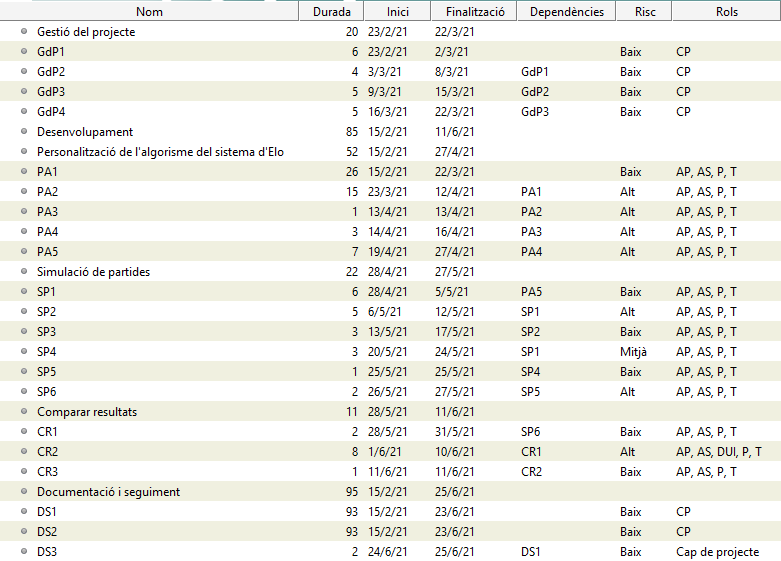
\includegraphics[width=1.15\textwidth]{images/GantEloEscrit.png}
    \caption{Diagrama de Gantt part textual}
    \label{fig:GanttText}
\end{figure}
 \newpage

        \begin{figure}[h!]
        \centering
            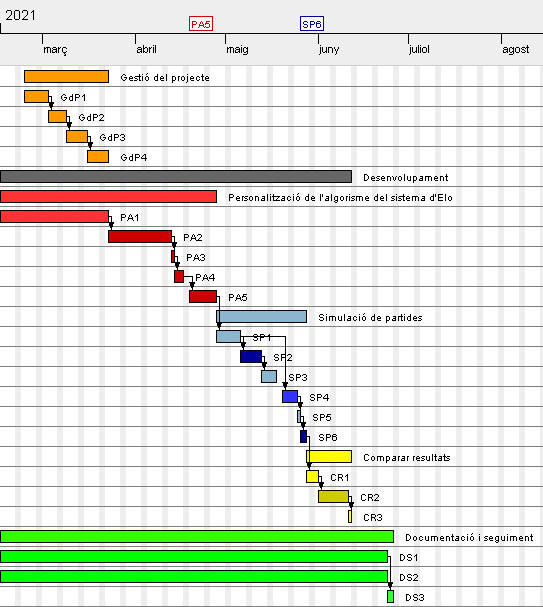
\includegraphics[width=1.05
            \textwidth]{images/GantElo.png}%
            \caption{Diagrama de Gantt del projecte part visual}
            \label{fig:GanttElo}
        \end{figure}
        
\section{Gestió del risc}
Durant el desenvolupament del projecte poden sortir un seguit de riscos que el poden afectar negativament, arribant a endarrerir les tasques programades o fins i tot haver-ne d'eliminar alguna per la falta de temps. És per aquest motiu que cal identificar-los bé i preparar plans alternatius per arribar a solucionar aquests problemes, per poder acabar el projecte a temps i amb totes les funcionalitats. A la taula \ref{tab:taulaRiscos} podem observar els diversos riscos considerats, junt amb la probabilitat de que passin i amb l'impacte que poden tenir sobr el treball.

\begin{table}[H]
    \begin{center}
        \begin{tabular}{ | c | c | c |}
              \rowcolor{lightgray} \hline \textbf{Risc} & \textbf{Probabilitat} & \textbf{Impacte} \\ \hline
              Data d'entrega fixa & Baixa & Alt \\ \hline
              Desconeixement en simulació & Alt & Baix \\ \hline
              Desconeixement en les tecnologies emprades & Alt & Baix \\ \hline
              Bugs i errors & Alt & Mig \\ \hline
        \end{tabular}
        \caption{Taula dels possibles riscos amb les seves probabilitats de que passin}
        \label{tab:taulaRiscos}
        \end{center}
\end{table}  

Ara que ja es coneixen els riscos i la seva probabilitat de que apareguin, s'explicaran els plans alternatius per solucionar-los.
\begin{itemize}
    \item \textbf{Data d'entrega fixa:} Com s'ha mostrat anteriorment, la probabilitat de que passi aquest risc és baixa, ja que tota la planificació s'ha fet pensant en la data màxima. Tot i així, pot arribar a tindre conseqüències molt greus, perquè en els pitjors dels casos es pot arribar a eliminar una funcionalitat de les proposades per arribar a l'entrega. Per evitar-ho, el que es farà serà fer una bona planificació tenint en compte tots els problemes i donant un marge de temps per poder-los solucionar. No farà falta cap recurs addicional.
    \item \textbf{Desconeixement en simulació:} Com es pot observar en la taula \ref{tab:taulaRiscos} prèviament vista, és molt probable que aparegui un problema degut al desconeixement que tinc sobre la simulació. Un pla alternatiu per solucionar-ho és afegir més hores de les necessàries a les respectives tasques per així no generar endarreriments. També es preguntarà al professor responsable de l'assignatura sobre algun dubte en concret. Aquest risc només tindrà un impacte baix, ja que només pot arribar a generar un endarreriment. No farà falta cap recurs addicional.
    \item \textbf{Desconeixement en les tecnologies emprades:} Com es pot veure en la taula \ref{tab:taulaRiscos}, la probabilitat de que surti un risc relacionat amb el desconeixement de les tecnologies emprades és molt alta. Aquest risc té un impacte mitjà ja que hi ha vàries tecnologies de les quals no tinc gaire coneixement i, per tant, poden generar diversos retards.  Per aquest motiu, s'estudiarà prèviament el seu funcionament i s'afegiran més hores de les necessàries a les tasques on s'utilitzin. No serà necessari cap recurs addicional.
    \item \textbf{Bugs i errors:} En el desenvolupament de tot programa informàtic, és molt habitual que apareguin bugs i errors a l'hora de desenvolupar i testejar. Per aquest motiu, la probabilitat de que passi en el projecte és molt alta i per solucionar-ho es faran tests unitaris. En cas de que alguna funcionalitat testejada doni un error més tard, se li dedicarà temps per trobar-lo i corregir-lo. L'impacte que pot arribar a tenir és el d'alentir el desenvolupament del projecte i no farà falta cap recurs addicional per corregir-lo.
\end{itemize}

\newpage
\section{Gestió econòmica}
\subsection{Identificació i estimació de costos}
Un aspecte molt important a tindre en compte a l'hora de desenvolupar un projecte és el pressupost. Per aquest motiu, s'han de valorar tots els costos possibles: recursos humans, recursos materials, recursos generals, contingència i imprevistos. 
Com s'ha explicat anteriorment, s'ha afegit una tasca des de la planificació inicial. Aquesta ha comportat el canvi d'hores destinades en les tasques afectades. Tot i això, el preu gairebé no ha canviat, ha variat en temes de pocs euros, per tant, ha estat un canvi insignificant. A continuació es calcularà cada un dels costos actualitzats i finalment es veurà el cost final del projecte.

\subsubsection{Recursos humans}
Com s'ha explicat prèviament, dintre dels recursos humans hi ha diferents rols. Aquests tenen funcions diferents i treballaran més o menys depenent de les tasques descrites prèviament en el diagrama de Gantt. Per tant, per poder saber el cost total del projecte, cal saber primer el seu sou. Aquest s'ha calculat fent la  mitjana dels sous que es mostren en la pàgina de Tecnoempleo.com \cite{tecnoEmpleo} i que podem veure a la taula \ref{tab:TaulaSouRols}. Aquesta conté els diversos rols, els seus salaris brut per hora i els mateixos tenint en compte la seguretat social (SS). 

\begin{table}[H]
    \begin{center}
        \begin{tabular}{|l|c|c|}
            \hline
            \rowcolor[HTML]{9B9B9B} 
            \multicolumn{1}{|c|}{\cellcolor[HTML]{9B9B9B}{\color[HTML]{000000} \textbf{Rol}}} & {\color[HTML]{000000} \textbf{Sou/hora (brut)}} & {\color[HTML]{000000} \textbf{Sou/hora + SS(x1,3) (brut)}} \\ \hline
            {\color[HTML]{000000} Cap de projecte}                                            & {\color[HTML]{000000} 23,54€}                   & {\color[HTML]{000000} 30,61€}                              \\ \hline
            {\color[HTML]{000000} Analista programador}                                       & {\color[HTML]{000000} 16,74€}                   & {\color[HTML]{000000} 21,77€}                              \\ \hline
            {\color[HTML]{000000} Arquitecte del Software}                                    & {\color[HTML]{000000} 20,77€}                   & {\color[HTML]{000000} 27€}                                 \\ \hline
            {\color[HTML]{000000} Dissenyador d'UI}                                           & {\color[HTML]{000000} 15,57€}                   & {\color[HTML]{000000} 20,24€}                              \\ \hline
            {\color[HTML]{000000} Programador}                                                & {\color[HTML]{000000} 15,51€}                   & {\color[HTML]{000000} 20,17€}                              \\ \hline
            {\color[HTML]{000000} Tester}                                                     & {\color[HTML]{000000} 15,40€}                   & {\color[HTML]{000000} 20,02€}                              \\ \hline
        \end{tabular}
        \caption{Taula dels sous per hora dels diferents rols del projecte}
        \label{tab:TaulaSouRols}
    \end{center}
\end{table}

Un cop coneguts els preus, ja es pot calcular el de cada tasca. Per fer-ho, es calcularà les hores necessàries de cada rol per cada una d'elles, mostrades anteriorment en el diagrama de Gannt. El cost total de les tasques es pot veure en la taula \ref{tab:TaulaCostosTasques}, on s'indica el nom de la feina a fer, i per cada una, les hores per cada respectiu rol, les hores totals de la tasca i el seu cost.

\begin{table}[H]
    \begin{center}
        \begin{tabular}{|l|c|c|c|c|c|c|c|c|}
            \hline
            \rowcolor[HTML]{9B9B9B} 
            {\color[HTML]{000000} \textbf{Tasca}}                                                  & {\color[HTML]{000000} \textbf{\begin{tabular}[c]{@{}c@{}}Hores \\ totals\end{tabular}}} & {\color[HTML]{000000} \textbf{CP}}        & {\color[HTML]{000000} \textbf{AP}}      & {\color[HTML]{000000} \textbf{AS}}   & {\color[HTML]{000000} \textbf{DUI}}     & {\color[HTML]{000000} \textbf{P}}         & {\color[HTML]{000000} \textbf{T}}       & {\color[HTML]{000000} \textbf{Cost}}       \\ \hline
            \rowcolor[HTML]{C0C0C0} 
            {\color[HTML]{000000} \textbf{GdP}}                                                    & {\color[HTML]{000000} \textbf{70}}                                                      & {\color[HTML]{000000} \textbf{}}          & {\color[HTML]{000000} \textbf{}}        & {\color[HTML]{000000} \textbf{}}     & {\color[HTML]{000000} \textbf{}}        & {\color[HTML]{000000} \textbf{}}          & {\color[HTML]{000000} \textbf{}}        & {\color[HTML]{000000} \textbf{}}           \\ \hline
            {\color[HTML]{000000} GdP1}                                                            & {\color[HTML]{000000} 25}                                                               & {\color[HTML]{000000} 25}                 & {\color[HTML]{000000} }                 & {\color[HTML]{000000} }              & {\color[HTML]{000000} }                 & {\color[HTML]{000000} }                   & {\color[HTML]{000000} }                 & {\color[HTML]{000000} 765,25€}             \\ \hline
            {\color[HTML]{000000} GdP2}                                                            & {\color[HTML]{000000} 10}                                                               & {\color[HTML]{000000} 10}                 & {\color[HTML]{000000} }                 & {\color[HTML]{000000} }              & {\color[HTML]{000000} }                 & {\color[HTML]{000000} }                   & {\color[HTML]{000000} }                 & {\color[HTML]{000000} 306,10€}             \\ \hline
            {\color[HTML]{000000} GdP3}                                                            & {\color[HTML]{000000} 15}                                                               & {\color[HTML]{000000} 15}                 & {\color[HTML]{000000} }                 & {\color[HTML]{000000} }              & {\color[HTML]{000000} }                 & {\color[HTML]{000000} }                   & {\color[HTML]{000000} }                 & {\color[HTML]{000000} 459,15€}             \\ \hline
            {\color[HTML]{000000} GdP4}                                                            & {\color[HTML]{000000} 20}                                                               & {\color[HTML]{000000} 20}                 & {\color[HTML]{000000} }                 & {\color[HTML]{000000} }              & {\color[HTML]{000000} }                 & {\color[HTML]{000000} }                   & {\color[HTML]{000000} }                 & {\color[HTML]{000000} 612,20€}             \\ \hline
            \rowcolor[HTML]{C0C0C0} 
            {\color[HTML]{000000} \textbf{D}}                                                      & {\color[HTML]{000000} \textbf{270}}                                                     & {\color[HTML]{000000} \textbf{}}          & {\color[HTML]{000000} \textbf{}}        & {\color[HTML]{000000} \textbf{}}     & {\color[HTML]{000000} \textbf{}}        & {\color[HTML]{000000} \textbf{}}          & {\color[HTML]{000000} \textbf{}}        & {\color[HTML]{000000} \textbf{}}           \\ \hline
            {\color[HTML]{000000} PA1}                                                             & {\color[HTML]{000000} 10}                                                               & {\color[HTML]{000000} }                   & {\color[HTML]{000000} 5}                & {\color[HTML]{000000} 3,5}           & {\color[HTML]{000000} }                 & {\color[HTML]{000000} 1}                  & {\color[HTML]{000000} 0,5}              & {\color[HTML]{000000} 233.53€}             \\ \hline
            {\color[HTML]{000000} PA2}                                                             & {\color[HTML]{000000} 50}                                                               & {\color[HTML]{000000} }                   & {\color[HTML]{000000} 5}                & {\color[HTML]{000000} 5}             & {\color[HTML]{000000} }                 & {\color[HTML]{000000} 35}                  & {\color[HTML]{000000} 5}                & {\color[HTML]{000000} 1049,90€}             \\ \hline
             {\color[HTML]{000000} PA3}                                                             & {\color[HTML]{000000} 5}                                                               & {\color[HTML]{000000} }                   & {\color[HTML]{000000} 0,5}                & {\color[HTML]{000000} 0,5}             & {\color[HTML]{000000} }                 & {\color[HTML]{000000} 3,5}                  & {\color[HTML]{000000} 0,5}                & {\color[HTML]{000000} 104,99€}             \\ \hline
            {\color[HTML]{000000} PA4}                                                             & {\color[HTML]{000000} 15}                                                               & {\color[HTML]{000000} }                   & {\color[HTML]{000000} 1}                & {\color[HTML]{000000} 1}             & {\color[HTML]{000000} }                 & {\color[HTML]{000000} 10,5}               & {\color[HTML]{000000} 2,5}              & {\color[HTML]{000000} 310,61€}             \\ \hline
            {\color[HTML]{000000} PA5}                                                             & {\color[HTML]{000000} 35}                                                               & {\color[HTML]{000000} }                   & {\color[HTML]{000000} 3}                & {\color[HTML]{000000} 3}             & {\color[HTML]{000000} }                 & {\color[HTML]{000000} 24,5}               & {\color[HTML]{000000} 4,5}              & {\color[HTML]{000000} 735,57€}             \\ \hline
            {\color[HTML]{000000} SP1}                                                             & {\color[HTML]{000000} 30}                                                               & {\color[HTML]{000000} }                   & {\color[HTML]{000000} 3}              & {\color[HTML]{000000} 3}           & {\color[HTML]{000000} }                 & {\color[HTML]{000000} 22,5}                 & {\color[HTML]{000000} 1,5}                & {\color[HTML]{000000} 630,17€}             \\ \hline
            {\color[HTML]{000000} SP2}                                                             & {\color[HTML]{000000} 25}                                                               & {\color[HTML]{000000} }                   & {\color[HTML]{000000} 2}              & {\color[HTML]{000000} 2}           & {\color[HTML]{000000} }                 & {\color[HTML]{000000} 18}                 & {\color[HTML]{000000} 3}                & {\color[HTML]{000000} 419,96}             \\ \hline
            {\color[HTML]{000000} SP3}                                                             & {\color[HTML]{000000} 15}                                                               & {\color[HTML]{000000} }                   & {\color[HTML]{000000} 1,5}                & {\color[HTML]{000000} 1,5}             & {\color[HTML]{000000} }                 & {\color[HTML]{000000} 10,5}                 & {\color[HTML]{000000} 1,5}                & {\color[HTML]{000000} 314,97€}             \\ \hline
            {\color[HTML]{000000} SP4}                                                             & {\color[HTML]{000000} 15}                                                               & {\color[HTML]{000000} }                   & {\color[HTML]{000000} 1,5}                & {\color[HTML]{000000} 1,5}             & {\color[HTML]{000000} }                 & {\color[HTML]{000000} 10,5}                 & {\color[HTML]{000000} 1,5}                & {\color[HTML]{000000} 314,97€}             \\ \hline
            {\color[HTML]{000000} SP5}                                                             & {\color[HTML]{000000} 5}                                                                & {\color[HTML]{000000} }                   & {\color[HTML]{000000} 0,5}              & {\color[HTML]{000000} 0,5}           & {\color[HTML]{000000} }                 & {\color[HTML]{000000} 3,5}                & {\color[HTML]{000000} 0,5}              & {\color[HTML]{000000} 104,99€}             \\ \hline
            {\color[HTML]{000000} SP6}                                                             & {\color[HTML]{000000} 10}                                                               & {\color[HTML]{000000} }                   & {\color[HTML]{000000} 1}                & {\color[HTML]{000000} 0,5}             & {\color[HTML]{000000} }                 & {\color[HTML]{000000} 7}                 & {\color[HTML]{000000} 1,5}                & {\color[HTML]{000000} 206,49€}             \\ \hline
            {\color[HTML]{000000} CR1}                                                             & {\color[HTML]{000000} 10}                                                               & {\color[HTML]{000000} }                   & {\color[HTML]{000000} 0,5}                & {\color[HTML]{000000} 1,5}             & {\color[HTML]{000000} }                 & {\color[HTML]{000000} 7}                 & {\color[HTML]{000000} 1}                & {\color[HTML]{000000} 212,60€}             \\ \hline
            {\color[HTML]{000000} CR2}                                                             & {\color[HTML]{000000} 40}                                                               & {\color[HTML]{000000} }                   & {\color[HTML]{000000} 2}                & {\color[HTML]{000000} 2}             & {\color[HTML]{000000} 18}               & {\color[HTML]{000000} 14}                 & {\color[HTML]{000000} 4}                & {\color[HTML]{000000} 824,32€}             \\ \hline
            {\color[HTML]{000000} CR3}                                                             & {\color[HTML]{000000} 5}                                                               & {\color[HTML]{000000} }                   & {\color[HTML]{000000} 0,5}                & {\color[HTML]{000000} 0,5}             & {\color[HTML]{000000} }                 & {\color[HTML]{000000} 3,5}                  & {\color[HTML]{000000} 0,5}                & {\color[HTML]{000000} 104,99€}             \\ \hline
            \rowcolor[HTML]{C0C0C0} 
            {\color[HTML]{000000} \textbf{DS}}                                                     & {\color[HTML]{000000} \textbf{110}}                                                     & {\color[HTML]{000000} \textbf{}}          & {\color[HTML]{000000} \textbf{}}        & {\color[HTML]{000000} \textbf{}}     & {\color[HTML]{000000} \textbf{}}        & {\color[HTML]{000000} \textbf{}}          & {\color[HTML]{000000} \textbf{}}        & {\color[HTML]{000000} \textbf{}}           \\ \hline
            {\color[HTML]{000000} DS1}                                                             & {\color[HTML]{000000} 75}                                                               & {\color[HTML]{000000} 75}                 & {\color[HTML]{000000} }                 & {\color[HTML]{000000} }              & {\color[HTML]{000000} }                 & {\color[HTML]{000000} }                   & {\color[HTML]{000000} }                 & {\color[HTML]{000000} 2295,75€}            \\ \hline
            {\color[HTML]{000000} DS2}                                                             & {\color[HTML]{000000} 25}                                                               & {\color[HTML]{000000} 25}                 & {\color[HTML]{000000} }                 & {\color[HTML]{000000} }              & {\color[HTML]{000000} }                 & {\color[HTML]{000000} }                   & {\color[HTML]{000000} }                 & {\color[HTML]{000000} 765,25€}             \\ \hline
            {\color[HTML]{000000} DS3}                                                             & {\color[HTML]{000000} 10}                                                               & {\color[HTML]{000000} 10}                 & {\color[HTML]{000000} }                 & {\color[HTML]{000000} }              & {\color[HTML]{000000} }                 & {\color[HTML]{000000} }                   & {\color[HTML]{000000} }                 & {\color[HTML]{000000} 306,10€}             \\ \hline
            \rowcolor[HTML]{C0C0C0} 
            {\color[HTML]{000000} \textbf{\begin{tabular}[c]{@{}l@{}}TOTAL \\ HORES\end{tabular}}} & {\color[HTML]{000000} \textbf{450}}                                                     & {\color[HTML]{000000} \textbf{180}}       & {\color[HTML]{000000} \textbf{27}}    & {\color[HTML]{000000} \textbf{26}}   & {\color[HTML]{000000} \textbf{18}}      & {\color[HTML]{000000} \textbf{171}}     & {\color[HTML]{000000} \textbf{28}}      & {\color[HTML]{000000} \textbf{}}           \\ \hline
            \rowcolor[HTML]{C0C0C0} 
            {\color[HTML]{000000} \textbf{\begin{tabular}[c]{@{}l@{}}TOTAL \\ COST\end{tabular}}}  & {\color[HTML]{000000} \textbf{}}                                                        & {\color[HTML]{000000} \textbf{5.509,80€}} & {\color[HTML]{000000} \textbf{587,79€}} & {\color[HTML]{000000} \textbf{702€}} & {\color[HTML]{000000} \textbf{364,32€}} & {\color[HTML]{000000} \textbf{3.449,07€}} & {\color[HTML]{000000} \textbf{560,56€}} & {\color[HTML]{000000} \textbf{11.173,54€}} \\ \hline
        \end{tabular}
        \caption{Taula dels costos de les tasques del projecte}
        \label{tab:TaulaCostosTasques}
    \end{center}
\end{table}

\subsubsection{Recursos materials}
Un altre aspecte a tenir en compte a l'hora de calcular el pressupost d'un projecte són els recursos materials. En aquest cas, s'utilitzarà un HP Laptop 15s-fq2093ns \cite{HPLaptop} durant tot el desenvolupament i un ratolí inalàmbric HP 220 \cite{HPRatoli}. Respecte els softwares que s'utilitzaran, hi han alguns que son de franc, com és el cas del Lua o el Github, i d'altres de pagament, com el Visual Studio o Qt.

A la taula \ref{tab:TaulaCostosHardware} es pot observar els recursos materials de hardware amb els seus costos, els seus anys de vida útil i les seves amortitzacions. Aquests càlculs estan fets sobre 4 anys de vida útil i amb una utilització de 5 hores diàries. La fórmula utilitzada pel càlcul de l'amortització és la següent:

\[
\frac{cost\, del\, hardware (euros)}{vida\, \acute{u}til (anys) * 220\, dies\, laborables/any * hores\, dedicades\, al\, dia} * durada\, del\, projecte (hores)
\]

\begin{table}[H]
    \begin{center}
        \begin{tabular}{|l|c|c|c|}
            \hline
            \rowcolor[HTML]{9B9B9B} 
            {\color[HTML]{000000} \textbf{Hardware}} & {\color[HTML]{000000} \textbf{Cost}} & {\color[HTML]{000000} \textbf{Vida útil}} & {\color[HTML]{000000} \textbf{Amortització}} \\ \hline
            HP Laptop 15s-fq2093ns                   & 650€                                 & 4 anys                                    & 66,48€                                       \\ \hline
            Ratolí inalàmbric HP 220                 & 20€                                  & 4 anys                                    & 2,05€                                        \\ \hline
            \rowcolor[HTML]{C0C0C0} 
            {\color[HTML]{000000} \textbf{Total}}    & {\color[HTML]{000000} \textbf{670€}}     & {\color[HTML]{000000} \textbf{}}          & {\color[HTML]{000000} \textbf{68,53€}}       \\ \hline
        \end{tabular}
        \caption{Taula dels costos dels recursos hardware i la seva amortització}
        \label{tab:TaulaCostosHardware}
    \end{center}
\end{table}

A la taula \ref{tab:TaulaCostosSoftware} es pot observar els recursos materials de software i els seus costos. Aquesta inclou la llicència de Windows \cite{Windows}, la del Visual Studio \cite{VisualStudio} i la de QT \cite{Qt}. Aquesta última s'ha de pagar per mesos durant tot un any.

\begin{table}[H]
    \begin{center}
        \begin{tabular}{|l|c|c|c|}
            \hline
            \rowcolor[HTML]{9B9B9B} 
            {\color[HTML]{000000} \textbf{Software}} & {\color[HTML]{000000} \textbf{Cost/mes}} & {\color[HTML]{000000} \textbf{Mesos}} & {\color[HTML]{000000} \textbf{Cost}} \\ \hline
            {\color[HTML]{000000} Windows}           & {\color[HTML]{000000} 145€}              & {\color[HTML]{000000} }               & {\color[HTML]{000000} 145€}          \\ \hline
            {\color[HTML]{000000} Visual Studio}     & {\color[HTML]{000000} 45€}               & {\color[HTML]{000000} 5}              & {\color[HTML]{000000} 225€}          \\ \hline
            {\color[HTML]{000000} QT}                & {\color[HTML]{000000} 42€}               & {\color[HTML]{000000} 12}             & {\color[HTML]{000000} 504€}          \\ \hline
            \rowcolor[HTML]{C0C0C0} 
            {\color[HTML]{000000} \textbf{Total}}    & {\color[HTML]{000000} \textbf{}}         & {\color[HTML]{000000} \textbf{}}      & {\color[HTML]{000000} \textbf{874€}} \\ \hline
        \end{tabular}
        \caption{Taula dels costos dels recursos hardware i la seva amortització}
        \label{tab:TaulaCostosSoftware}
    \end{center}
\end{table}

Finalment, a la taula \ref{tab:TaulaCostosMaterials} podem observar el cost total dels recursos materials.

\begin{table}[H]
    \begin{center}
        \begin{tabular}{|l|c|}
            \hline
            \rowcolor[HTML]{9B9B9B} 
            {\color[HTML]{000000} \textbf{Recurs material}} & {\color[HTML]{000000} \textbf{Cost}}  \\ \hline
            {\color[HTML]{000000} Hardware}                 & {\color[HTML]{000000} 670€}           \\ \hline
            {\color[HTML]{000000} Software}                 & {\color[HTML]{000000} 874€}           \\ \hline
            \rowcolor[HTML]{C0C0C0} 
            {\color[HTML]{000000} \textbf{Total}}           & {\color[HTML]{000000} \textbf{1554€}} \\ \hline
        \end{tabular}
        \caption{Taula dels costos dels recursos hardware i la seva amortització}
        \label{tab:TaulaCostosMaterials}
    \end{center}
\end{table}

\subsubsection{Recursos generals}
A part dels recursos humans i materials, per poder calcular el pressupost sencer del projecte també s'han de tindre en compte altres elements com l'Internet, l'electricitat, el desplaçament, l'espai de treball, etc. En aquest cas, el treball és desenvolupat per una sola persona des de casa, per tant, només es contemplaran els dos primers costos. Per l'electricitat, es tindran en compte dos llums LEDs que consumeixen 14 W i l'ordinador que consum 150 W. A la taula \ref{tab:TaulaCostosGenerals} es pot veure el cost dels diversos recursos generals.

\begin{table}[H]
    \begin{center}
        \begin{tabular}{|l|c|c|}
            \hline
            \rowcolor[HTML]{9B9B9B} 
            {\color[HTML]{000000} \textbf{Recursos}} & {\color[HTML]{000000} \textbf{Cost}} & {\color[HTML]{000000} \textbf{Cost Total}} \\ \hline
            Electricitat                             & 0,1458€/kWh                          & 11,68€                                     \\ \hline
            Internet                                 & 48,40€/mes                           & 193,60€                                    \\ \hline
            \rowcolor[HTML]{C0C0C0} 
            {\color[HTML]{000000} \textbf{Total}}    & {\color[HTML]{000000} \textbf{}}     & {\color[HTML]{000000} \textbf{205,28€}}    \\ \hline
        \end{tabular}
        \caption{Taula dels costos dels recursos generals}
        \label{tab:TaulaCostosGenerals}
    \end{center}
\end{table}

\subsubsection{Contingència}
Un altre aspecte a tenir present és la contingència, és a dir, és un cost que se li suma al pressupost per cobrir aquells imprevists que no s'han anticipat. Aquesta es calcula amb un percentatge del cost dels recursos calculats. En el sector informàtic, aquest percentatge varia entre el 10\% i el 20\%, per tant, s'escollirà el punt mig, és a dir, el 15\%. A la taula \ref{tab:TaulaContingència} podem observar la taula de contingència pels diferents recursos calculats anteriorment.

\begin{table}[H]
    \begin{center}
        \begin{tabular}{|l|c|c|c|}
            \hline
            \rowcolor[HTML]{9B9B9B} 
            {\color[HTML]{000000} \textbf{Tipus de recursos}} & {\color[HTML]{000000} \textbf{Cost}} & {\color[HTML]{000000} \textbf{\% de Contingència}} & {\color[HTML]{000000} \textbf{Cost contingència}} \\ \hline
            {\color[HTML]{000000} Recursos humans}            & {\color[HTML]{000000} 11.173,54€}    & {\color[HTML]{000000} }                            & {\color[HTML]{000000} 1.676,04€}                  \\ \cline{1-2} \cline{4-4} 
            {\color[HTML]{000000} Recursos materials}         & {\color[HTML]{000000} 1544€}          & {\color[HTML]{000000} }                            & {\color[HTML]{000000} 231,60€}                    \\ \cline{1-2} \cline{4-4} 
            {\color[HTML]{000000} Recursos generals}          & {\color[HTML]{000000} 205,28€}       & \multirow{-3}{*}{{\color[HTML]{000000} 15\%}}      & {\color[HTML]{000000} 30,72€}                     \\ \hline
            \rowcolor[HTML]{C0C0C0} 
            {\color[HTML]{000000} \textbf{Total}}             & {\color[HTML]{000000} \textbf{}}     & {\color[HTML]{000000} \textbf{}}                   & {\color[HTML]{000000} \textbf{1.938,36€}}         \\ \hline
        \end{tabular}
        \caption{Taula de contingència dels diversos recursos}
        \label{tab:TaulaContingència}
    \end{center}
\end{table}

\subsubsection{Cost d'imprevistos}
Finalment, cal calcular el cost de tots aquells imprevistos que s'han identificat prèviament en l'apartat de riscos. A la taula \ref{tab:TaulaImprevistos} podem veure el cost de cada un d'ells junt amb la seva probabilitat de que passin.

\begin{table}[H]
    \begin{center}
        \begin{tabular}{|l|c|c|c|}
            \hline
            \rowcolor[HTML]{9B9B9B} 
            {\color[HTML]{000000} \textbf{Risc}}                                                                       & {\color[HTML]{000000} \textbf{Probabilitat}} & {\color[HTML]{000000} \textbf{Temps}} & {\color[HTML]{000000} \textbf{Cost}}    \\ \hline
            {\color[HTML]{000000} Data entrega fixa}                                                                   & {\color[HTML]{000000} 10\%}                  & {\color[HTML]{000000} 10 hores}       & {\color[HTML]{000000} 30,61€}           \\ \hline
            {\color[HTML]{000000} \begin{tabular}[c]{@{}l@{}}Desconeixement\\ en simulació\end{tabular}}               & {\color[HTML]{000000} 66\%}                  & {\color[HTML]{000000} 10 hores}       & {\color[HTML]{000000} 133,12€}          \\ \hline
            {\color[HTML]{000000} \begin{tabular}[c]{@{}l@{}}Desconeixement \\ en tecnologies\\ emprades\end{tabular}} & {\color[HTML]{000000} 66\%}                  & {\color[HTML]{000000} 15 hores}       & {\color[HTML]{000000} 199,68€}          \\ \hline
            {\color[HTML]{000000} Bugs i errors}                                                                       & {\color[HTML]{000000} 66\%}                  & {\color[HTML]{000000} 20 hores}       & {\color[HTML]{000000} 264,26€}          \\ \hline
            \rowcolor[HTML]{C0C0C0} 
            {\color[HTML]{000000} \textbf{Total}}                                                                      & {\color[HTML]{000000} \textbf{}}             & {\color[HTML]{000000} \textbf{}}      & {\color[HTML]{000000} \textbf{627,67€}} \\ \hline
        \end{tabular}
        \caption{Taula del cost d'imprevistos}
        \label{tab:TaulaImprevistos}
    \end{center}
\end{table}

\subsubsection{Pressupost final}

Un cop ja s'han calculat tots els càlculs necessaris dels diferents costos, ja es pot determinar el pressupost final que costarà el projecte. Aquest el podem veure en la taula \ref{tab:TaulaFinal}, on si arrodonim el preu a l'alça, queda amb un total de 15.489€, gairebé 15.500€.

\begin{table}[H]
    \begin{center}
        \begin{tabular}{|l|c|}
            \hline
            \rowcolor[HTML]{9B9B9B} 
            {\color[HTML]{000000} \textbf{}}          & {\color[HTML]{000000} \textbf{Cost}}       \\ \hline
            {\color[HTML]{000000} Recursos humans}    & {\color[HTML]{000000} 11.173,54€}          \\ \hline
            {\color[HTML]{000000} Recursos materials} & {\color[HTML]{000000} 1544€}                \\ \hline
            {\color[HTML]{000000} Recursos generals}  & {\color[HTML]{000000} 205,28€}             \\ \hline
            {\color[HTML]{000000} Contingència}       & {\color[HTML]{000000} 1.938,36€}           \\ \hline
            {\color[HTML]{000000} Imprevistos}        & {\color[HTML]{000000} 627,67€}             \\ \hline
            \rowcolor[HTML]{C0C0C0} 
            {\color[HTML]{000000} \textbf{Total}}     & {\color[HTML]{000000} \textbf{15.488,85€}} \\ \hline
        \end{tabular}
        \caption{Taula de pressupost final}
        \label{tab:TaulaFinal}
    \end{center}
\end{table}

\subsection{Control de gestió}

Planificar i gestionar el pressupost d'un projecte és molt important, però també s'ha de gestionar els diners i calcular les desviacions econòmiques per cadascuna de les tasques o costos calculats prèviament. Per fer-ho, per cada una de les tasques fetes, s'anotarà les hores reals que han estat necessàries i s'empraran les següents fórmules.
\begin{itemize}
    \item \textbf{Desviació d'hores per tasca}
    \[(Hores\,estimades - Hores\,reals)\]
    \item \textbf{Desviació de costos per tasca}
    \[(Hores\,estimades - Hores\,reals) * Cost\,real\]
    \item \textbf{Desviació d'hores dels recursos humans per cada tasca}
    \[(Hores\,estimades - Hores\,reals)\]
    \item \textbf{Desviació dels costos de recursos humans per cada tasca}
    \[(Cost\, estimat - Cost\,real) * Hores\,reals\]
    \item \textbf{Desviació total de recursos humans}
    \[Costos\,recursos\,humans\,estimats - Costos\,recursos\,humans\,reals\]
    \item \textbf{Desviació total de recursos materials}
    \[Costos\,recursos\,materials\,estimats - Costos\,recursos\,materials\,reals\]
    \item \textbf{Desviació total de recursos generals}
    \[Costos\,recursos\,generals\,estimats - Costos\,recursos\,generals\,reals\]
    \item \textbf{Desviació total de contingències}
    \[Cost\,contingència\,estimat - Cost\,contingència\,real\]
    \item \textbf{Desviació total d'imprevistos}
    \[Costos\,imprevistos\,estimats - Costos\,imprevistos\,reals\]
    \item \textbf{Desviació total d'hores}
    \[Hores\,estimades - Hores\,reals\]
    \item \textbf{Desviació total de pressupost final}
    \[Pressupost\,final\,estimat - Pressupost\,final\,real\]
\end{itemize}

\newpage
\section{Informe de sostenibilitat}
\subsection{Autoavaluació}
Després de realitzar l'enquesta sobre la sostenibilitat d'EDINSOST, m'he adonat que hi han aspectes que encara no conec i haig d'aprendre. Aquesta enquesta tracta  tres grans temes: el el mediambiental, el social i l'econòmic.

Pel que fa al primer tema, prèviament en la carrera ens han mostrat i explicat l'impacte del hardware obsolet i els cementiris tecnològics en els països subdesenvolupats, i totes les conseqüències que tenen per a la societat d'allà. En canvi, en cap moment ens han explicat la manera de mesurar aquests impactes ambientals i com evitar-los o reduir-los el més mínim possible.

Respecte el segon gran tema, el social, també ens han explicat diversos aspectes. Sé que un programa ha de ser ètic, equitatiu, ha de poder ser utilitzat per tothom i ha de ser transparent i, a més, també ha de ser beneficiós per a la societat. Un programa ha d'estar dissenyat per ajudar a la gent i facilitar-los la vida. És per aquest motiu que s'ha de pensar en totes les conseqüències directes i indirectes que tindrà en la societat, tot i que no sempre es fa. Finalment, torna a passar la mateixa situació que abans, en cap moment ens han explicat com mesurar com de gran és la contribució per a la societat.

Per acabar, respecte l'últim tòpic, l'econòmic, només conec el que s'ha explicat en algunes assignatures prèvies i en GEP. Sé com planificar un projecte, calcular el seu pressupost, tindre en compte els imprevistos o analitzar la competència per veure les necessitats que falten. Malauradament, encara no he pogut posar en pràctica els meus coneixements en un projecte que no estigui dintre del mon acadèmic.

En conclusió, tot i tindre consciència sobre diversos aspectes de sostenibilitat, encara em falta molt per aprendre i, el que és més important, aplicar-los al desenvolupament dels projectes. Combinar tots tres temes és una tasca complicada que s'ha d'intentar fer pel bé de tots.

\subsection{Dimensió ambiental}

\setlength{\parindent}{0cm}

\textbf{Has estimat l'impacte ambiental que tindrà la realització del projecte? T'has plantejat minimitzar l'impacte, per exemple, reutilitzant recursos?}

A l'hora de plantejar el projecte no es va pensar en l'impacte ambiental que tindria. Afortunadament, es tracte d'un software, i per tant, d'un material no físic. Els únics impactes ambientals que poden haver-hi són el de consum de llum, els recursos materials necessaris per desenvolupar el projecte i el desplaçament dels treballadors. Per sort, aquest és un treball realitzat per una sola persona des de casa, per la qual cosa no hi ha desplaçament. Els recursos materials son reutilitzats, ja que s'han utilitzat els que ja tenia prèviament, per tant, no n'ha fet falta comprar-ne cap de nou. Llavors, l'únic impacte que hi ha és el consum de llum.

\newpage

\textbf{Com es resolen actualment el problema que vols abordar(estat de l'art)? En què millorarà ambientalment la teva solució amb les existents?}

Actualment, com s'ha explicat prèviament, el problema es resol plantejant una simulació que s'adeqüi a l'algorisme d'Elo que es vol testejar i executant diverses partides. Per això, cal desenvolupar una versió diferent cada vegada que es canvia la fórmula, i per tant, equival a més temps i més consum d'energia. En canvi, el meu projecte no necessita una versió diferent cada vegada que es canvia l'algorisme de l'Elo, i per tant, estalvia més energia.

\subsection{Dimensió econòmica}

\textbf{Has estimat el cost de la realització del projecte (recursos humans i materials)?}

Durant la planificació de tot el projecte, s'ha fet un càlcul del pressupost necessari pel seu desenvolupament, on s'han tingut en compte els diversos recursos humans, materials i generals, a l'igual que les contingències i els imprevistos.

\textbf{Com es resolen actualment el problema que vols abordar (estat de l'art)? En què millorarà econòmicament la teva solució de les existents?}

Com s'ha explicat abans, el problema actualment es resol plantejant una simulació que s'adeqüi a l'algorisme d'Elo que es vol testejar i executant diverses partides. La millora econòmica que aporta el meu projecte és la de reducció de temps a l'hora de desenvolupar el videojoc, i per tant, menys personal que pagar. Per una altre part, gràcies a l'eina a desenvolupar, es podrà saber si el sistema d'Elo és el desitjat i per tant, el que es vol per millorar l'experiència del jugador. D'aquesta manera, si el joc té èxit, també es vendrà més i es generaran més beneficis. 

\subsection{Dimensió social}

\textbf{Què creus que t'aportarà a nivell personal la realització d'aquest projecte?}

La realització d'aquest projecte m'aportarà un gran coneixement i experiència sobre els llenguatges i les eines que utilitzaré per desenvolupar-ho. També em servirà per veure com funcionen els projectes petits i com de similar o diferent pot ser la planificació de la realitat.

\textbf{Com es resolen actualment el problema que vols abordar (estat de l'art)? En què millorarà socialment (qualitat de vida) la teva solució de les existents?}

Com ja s'ha dit abans, actualment el problema es resol plantejant una simulació que s'adeqüi a l'algorisme d'Elo que es vol testejar i executant diverses partides. Gràcies al projecte, els treballadors hauran de pensar menys en com desenvolupar una simulació per cada fórmula i els jugadors podran gaudir més dels videojocs gràcies a que tenen el sistema d'Elo desitjat per l'empresa. 

\newpage

\textbf{Existeix una necessitat real del projecte?}

Realment si existeix una necessitat real. Com es va dir prèviament, els videojocs cada vegada són més famosos i tenen un impacte més important en la societat. Per tant, desenvolupar un bon joc és molt important, i una de les claus en fer-ho, es fer un bon sistema d'Elo, per a que els jugadors ho gaudeixin. Per tant, aquest programa ajuda a que això passi, i a més, estalvia temps de desenvolupament.

\newpage
\section{Lleis i regulacions}
A l'hora de fer un programa informàtic és molt important complir les lleis i satisfer les regulacions. L'incompliment d'una d'elles pot provocar greus conseqüències que poden ser penalitzades de forma molt severa. 

Si revisem el funcionament del meu programa, es pot arribar a la conclusió de què no vulnera cap llei ni incompleix cap legislació. Totes les dades utilitzades són creades de forma aleatòria o introduïdes pel propi usuari, i únicament són utilitzades per fer les simulacions. En cap moment són emmagatzemades en cap base de dades ni s'utilitza cap nom real, degut a que els jugadors funcionen amb IDs, no amb noms. 
Per una altra banda, el meu projecte tampoc té connexió a Internet. Com a resultat, no hi ha cap llei o regulació a vulnerar amb aquest aspecte. Finalment, l'ús del programa tampoc està restringit a cap edat. Si no és utilitzat amb l'objectiu d'estudiar una fórmula d'Elo particular, l'únic resultat que trobarà l'usuari serà un Excel amb la simulació executada, el qual no generarà cap risc ni inconvenient pel consumidor.

Pels motius que s'acaben d'explicar, es pot concloure que el meu TFG no vulnera cap llei ni regulació i tampoc està lligat a cap d'elles.

\newpage
%\section{Conclusions}
%\subsection{Conneixements aplicats d'assignatures prèvies}
\section{Conneixements aplicats d'assignatures prèvies}
Durant el desenvolupament d'aquest projecte s'han aplicat un gran nombre de coneixements apresos en les diverses assignatures de la carrera. A continuació, es faran menció a les matèries que més impacte han tingut:
\begin{itemize}
    \item \textbf{PRO1 i PRO2:} Aquestes dues assignatures han servit per conèixer els conceptes bàsics de la programació i per aprendre el llenguatge de C++, el qual ha estat utilitzat per desenvolupar el programa.
    \item \textbf{IDI:} Assignatura que m'ha servit per saber com s'ha de fer una interfície gràfica i quines característiques ha de tenir.
    \item \textbf{IES:} Matèria que m'ha ensenyat a fer i interpretar els diagrames de classe, a identificar les històries d'usuari i a tindre més coneixement sobre la jerarquia de classes.
    \item \textbf{PROP:} Aquesta assignatura m'ha servit per veure com es desenvolupa un projecte de grans dimensions i per a saber utilitzar GitHub.
    \item \textbf{ER:} Aquesta matèria m'ha servit per saber identificar els \textit{stakeholders} que té el sistema i els requisits que ha de complir. També m'ha ajudat a coneixer quins elements ha de tindre un document i com s'han de redactar.
    \item \textbf{AS:} L'assignatura d'AS m'ha servit per profunditzar sobre els diagrames de classe, per conèixer els patrons de disseny i per aprendre a fer tests unitaris.
    \item\textbf{GPS:} Aquesta matèria ha estat molt útil per saber com planificar un projecte i per tenir coneixement sobre les diverses metodologies que hi ha en el món laboral. Ha estat especialment útil per fer el curset de GEP.
    \item \textbf{PES:} PES ha estat l'assignatura que més ha aportat, i per tant, la més important. En aquesta matèria es desenvolupa un projecte sencer, des de l'estudi i planificació d'aquest fins a la seva realització. Com es pot veure, té molta similitud amb el TFG, i per tant, et prepara per aquest.
    \item \textbf{VJ:} Aquesta assignatura ha ajudat a augmentar el meu coneixement sobre el C++ après al principi de la carrera.
\end{itemize}

\begin{comment}

\subsubsection{Assoliment de les competències seleccionades}
\subsubsection*{CES1.1: Desenvolupar, mantenir i avaluar sistemes i serveis software complexos i/o crítics}
\subsubsection*{CES1.2: Donar solució a problemes d'integració en funció de les estratègies, dels estàndards i de les tecnologies disponibles}
\subsubsection*{CES1.3: Identificar, avaluar i gestionar els riscos potencials associats a la construcció de software que es poguessin presentar}
\subsubsection*{CES1.7: Controlar la qualitat i dissenyar proves en la producció de software}
\subsubsection*{CES2.1: Definir i gestionar els requisits d'un sistema software}

\end{comment}

\newpage
\nocite{*}
\printbibliography[heading=bibintoc]
\end{document}
